\documentclass[
 %reprint,
 aps, pra,
 amsmath,amssymb,
 11pt,
 final,
% notitlepage,
tightenlines,
 twoside,
 twocolumn,
 nofloats,
% nobibnotes,
nofootinbib,
 superscriptaddress,
%noshowpacs,
showkeys,
showkeywords,
%centertags
 ]
{revtex4-2}
\usepackage{subfigure}
\usepackage[font={small}]{caption}
\usepackage[T2A]{fontenc}
\usepackage{amsmath}
\usepackage[utf8]{inputenc}
\usepackage[russian,english]{babel}
\usepackage{graphicx}% Include figure files
\usepackage{dcolumn}% Align table columns on decimal point
\usepackage{bm}% bold math
\usepackage{xcolor}

\input{maik.rty}

%\renewcommand{\rmdefault}{lh}

\setcitestyle{authoryear,round}
\setlength{\bibhang}{1.5em}
\input{sao_cmd_author.tex}

\newcommand{\as}[1]{{\color{blue} #1}}
\newcommand{\tk}[1]{{\color{red} #1}}
\newcommand{\sao}{Специальная \as{астрофизическая} обсерватория
	РАН, Санкт-Петербург, 196140 Россия}
	
\begin{document}

\selectlanguage{russian}

\keywords{Солнце --- активные области --- корона --- магнитные поля --- радиоизлучение}

%\ydk{}
%\titlerunning{}
%\authorrunning{}
%\toctitle{}
%\tocauthor{}

\title{Определение высотного профиля температуры над активной областью на Солнце по результатам многочастотных радионаблюдений}

\author{\firstname{Т.~И.}~\surname{Кальтман}}
 \affiliation \sao

\author{\firstname{А.~Г.}~\surname{Ступишин}}
 \email{agstup@yandex.ru}
 \affiliation \sao

\author{\firstname{Г.~А.}~\surname{Макоев}}
 % \email{germanmakoev@gmail.com}
 \affiliation \sao

%----------------------------------------------------------------------------------------------------------------
\begin{abstract}
Представлен итерационный метод восстановления температурно-высотного профиля атмосферы Солнца над солнечным пятном по данным многочастотных спектро-поляризационных микроволновых наблюдений. Предполагается, что излучение формируется преимущественно в условиях гирорезонансного механизма на гармониках гирочастоты, а вклад на каждой частоте связан со слоем с оптической толщиной порядка единицы. Частотно-высотное соответствие определяется на основе экстраполяции фотосферного магнитного поля в корону. Восстановление профиля сведено к решению переопределённой системы линейных уравнений с регуляризацией, обеспечивающей устойчивость к шуму и физическую гладкость профиля. Метод протестирован на синтетических данных для дипольной модели пятна и применён к наблюдениям активной области NOAA 11312, выполненным на радиотелескопе РАТАН-600. Полученные температурные профили согласуются с современными моделями активных областей и воспроизводят наблюдаемые спектры в диапазоне 3–18 ГГц с точностью до нескольких процентов.
\end{abstract}

\maketitle
%\tableofcontents

\section{ВВЕДЕНИЕ}

Активные области представляют собой области концентрации сильных и устойчивых магнитных полей в атмосфере Солнца \citep{Solanki2003}. Магнитное поле определяет стратификацию плазмы и термодинамический режим от фотосферы до короны, подавляя конвекцию в нижних слоях и направляя теплопроводность вдоль силовых линий в переходной области и короне \citep{Solanki2006,Borrero2011}. В результате над солнечными пятнами формируется характерный вертикальный профиль температуры, существенно отличающийся от спокойной атмосферы.

В устойчивых (невспышечных) активных областях в переходной области и нижней короне устанавливается квазистационарный баланс между нагревом, теплопроводностью и радиационными потерями \citep{Aschwanden2005}. Этот энергетический баланс определяет температурно-высотное распределение плазмы. Поэтому восстановление вертикального профиля температуры является ключевой наблюдательной задачей для диагностики физических условий и механизмов нагрева короны.


Традиционно температурно-высотная структура атмосферы реконструируется по спектрам в крайнем ультрафиолетовом и рентгеновском диапазонах и на основе полуэмпирических моделей \citep{Vernazza1981,Maltby1986,Fontenla2009}. Однако в переходной области такие подходы осложнены нарушением локального термодинамического равновесия, неопределённостью оптической толщины и интегрированием по лучу зрения и высокой чувствительностью энергетического баланса к граничным условиям и параметризации нагрева \citep{Aschwanden2005}. Нелинейная зависимость теплопроводности и радиационных потерь от температуры делает задачу плохо обусловленной \citep{Spitzer1962}. На корональных высотах преимущественно восстанавливается распределение плазмы по температуре  ---  дифференциальная мера
эмиссии (DEM), 
тогда как переход к геометрической высоте требует дополнительных предположений, а чувствительность к магнитному полю остаётся ограниченной. Это мотивирует использование альтернативных диагностических методов.

Несмотря на развитие наблюдательной техники, вертикальная температурная структура над активными областями остаётся недостаточно определённой. Температура не измеряется напрямую и восстанавливается по спектральным характеристикам излучения с использованием инверсных и модельно-зависимых методов \citep{HannahKontar2012,Cheung2015}. Такие методы чувствительны одновременно к нескольким параметрам среды --- плотности, ионизационному состоянию и магнитному полю \citep{Zanna2018,Reale2014}, что приводит к неоднозначности интерпретации. Дополнительную сложность создаёт интегральный характер наблюдений вдоль луча зрения, особенно в переходной области и нижней короне, где существуют значительные высотные градиенты температуры и плотности \citep{Judge2010,Slemzin2014,Antonucci2020}.

Микроволновый диапазон обладает рядом преимуществ. В приближении закона Рэлея–Джинса яркостная температура непосредственно связана с кинетической температурой плазмы, что позволяет проводить количественную диагностику \citep{Dulk1985,Gary2004,Lee2007,Shibasaki2011}. Микроволновое излучение чувствительно как к температуре и плотности (свободно–свободный механизм), так и к магнитному полю (гирорезонансный механизм) \citep{Dulk1985,Shibasaki2011,Nindos2020}. В активных областях излучение в диапазоне нескольких гигагерц формируется преимущественно на гармониках гирочастоты, что обеспечивает естественную связь между частотой наблюдения, напряжённостью магнитного поля и высотой формирования \citep{1968SvA....12..245Z,1968SvA....12..464Z,1979SvA....23..316G,1980A&A....82...30A,1996ASSL..204.....Z}. Это делает микроволновые спектры перспективным инструментом восстановления температурно-высотной структуры над пятнами.

В работе \cite{Stupishin2018} был предложен итерационный метод согласования модельного и наблюдаемого спектров путём последовательного уточнения температурного профиля. Однако используемая схема требовала более строгой математической формализации, анализа устойчивости и обоснованной процедуры регуляризации.

В настоящей работе представлена формализованная версия итерационного метода восстановления температурно-высотного профиля по микроволновым спектро-поляризационным наблюдениям радиотелескопа РАТАН-600 \citep{Parijskij1993,Bogod2011,Bogod2023}. Рассматривается однородная по горизонтали модель атмосферы, в которой параметры зависят только от высоты, что позволяет исследовать свойства метода в контролируемых условиях и подготовить основу для дальнейшего усложнения модели. В отличие от параметризованных подходов с заданием закона нагрева \citep{Fleishman2021_Heating_Law}, температурный профиль не задаётся априорно.

Метод тестируется на синтетических данных для дипольной модели солнечного пятна, а затем применяется к наблюдениям активной области AR~NOAA~11312. Анализируются сходимость алгоритма, его чувствительность к входным параметрам и согласие восстановленного профиля с современными моделями солнечной атмосферы.
%================================================================================================================
\section{МЕТОДИКА}
\label{sec:method}
%----------------------------------------------------------------------------------------------------------------
\subsection{Физические и наблюдательные  основы}
%{\todo
%\begin{itemize}
%  \item Предположения: термодинамическое равновесие, %приближение Рэлея–Джинса.
%  \item Основной механизм: гирорезонансное излучение на 2-й\range4-й гармониках.
%  \item РАТАН-600: Используемые диапазоны частот (3\range18~ГГц), правая/левая круговая поляризация, пространстенное разрешение. Подходит под эту задачу.
%\end{itemize}
%}

Метод восстановления температурно-высотной структуры атмосферы
основан на свойствах микроволнового излучения активных областей
и особенностях его формирования в магнитной плазме.

В микроволновом диапазоне выполняется приближение Рэлея–Джинса,
в котором интенсивность $I_\nu$ связана с яркостной температурой $T_b$:
\begin{equation}
T_b = \frac{c^2}{k\nu^2}\, I_\nu ,
\end{equation}
где $c$ --- скорость света, $k$ --- постоянная Больцмана,
$\nu$ --- частота. В этих условиях $T_b$ непосредственно
характеризует кинетическую температуру электронов
в области формирования излучения.

В микроволновом диапазоне основным механизмом излучения
над пятнами является гирорезонансный (циклотронный) процесс,
возникающий при выполнении условия
\begin{equation}
\nu \approx s\,\nu_B =
s\,\frac{eB}{2\pi m_e c},
\end{equation}
где $\nu_B$ --- электронная гирочастота, $B$ --- напряжённость
магнитного поля, $e$ и $m_e$ --- заряд и масса электрона,
$s$ --- номер гармоники.
В активных областях наибольший вклад дают
\as{вторая и третья гармоники, в некоторых случаях возможен вклад четвертой гармоники}.

Поскольку магнитное поле убывает с высотой,
разные частоты формируются на различных уровнях атмосферы,
что обеспечивает связь частоты наблюдения с высотой формирования
и делает микроволновый спектр чувствительным
к вертикальной структуре температуры и магнитного поля.

Для реализации метода необходимы многочастотные
спектро-поляризационные наблюдения.
Регистрация правой и левой круговых поляризаций
позволяет учитывать различие условий формирования
излучения в обыкновенной и необыкновенной модах
и тем самым повышает диагностическую информативность.

В работе используются наблюдения радиотелескопа РАТАН-600 в диапазоне $3$\,--\,$18$~ГГц. Несмотря на одномерный и частотно-зависимый характер пространственного разрешения, широкий частотный диапазон наблюдений, спектральная дискретизация, регистрация правой и левой круговых поляризаций и высокая чувствительность инструмента обеспечивают достаточную диагностическую информативность для решения задачи восстановления температурно-высотной структуры в принятом приближении.


Предлагаемый подход не ограничен наблюдениями РАТАН-600
и  в дальнейшем может
быть обобщён на двумерные данные
интерферометрических инструментов
(SRH, EOVSA и др.).




\subsection{Модель атмосферы}
%{\todo
%\begin{itemize}
%  \item Принцип: плоско-слоистая атмосфера, один температурный профиль.
%  \item Разбиение по высоте, определение слоёв с оптической толщиной $\tau \approx 1$.
%  \item Система уравнений.
%\end{itemize}
%}

Для тестирования метода в контролируемых условиях вводится однородная плоскослоистая модель атмосферы,
в которой параметры плазмы зависят только от высоты $h$. 
В слоях формирования микроволнового излучения
предполагается локальное термодинамическое равновесие,
так что яркостная температура характеризует
электронную температуру плазмы.

Атмосфера дискретизируется на $M$ горизонтальных слоёв
с высотами $h_i$ (от уровня фотосферы), температурой $T_i$ и электронной плотностью $N_i$.
Шаг по высоте задаётся как входной параметр:
в области резкого температурного градиента
он уменьшается, а в квазиизотермических слоях увеличивается.


Распределение электронной плотности по высоте $h$ выше некоторой высоты $h_0$
задаётся барометрическим законом
(\cite{Aschwanden2005}, \S~3.1):
\begin{equation}
N(h) = N(h_0)\,\frac{T(h_0)}{T(h)}
\exp\!\left(-\frac{h-h_0}{\lambda T(h)}\right),
\label{barometric}
\end{equation}
где $\lambda = 4.7 \times 10^3 \,\mathrm{cm\,K^{-1}}$; 
формула применима при высотах, много меньших радиуса Солнца.

Для слоя между $h_1$ и $h_2$ вклад в поток на частоте $\nu$ в \as{круговой поляризации $p$
(правой (RCP) или левой (LCP))} определяется оптической толщиной
\begin{equation}
\tau_{\nu,p} = \int_{h_1}^{h_2}
\kappa_{\nu,p}(h)\,dh,
\end{equation}
где $\kappa_{\nu,p}$ --- коэффициент поглощения, зависящий от параметров плазмы и частоты.

Основной вклад в излучение на данной частоте
вносит слой, для которого $\tau_{\nu,p} \sim 1$,
что задаёт связь между частотой и характерной высотой формирования.

Модельный поток рассчитывается на основе
синтетических радиокарт, моделирующих
пространственное распределение яркости.
Карты свёртываются с диаграммой направленности
РАТАН-600, после чего получаются одномерные сканы,
сравниваемые с наблюдаемыми спектрами
в точке максимума. \as{<<Сканы, сравниваемые со спектрами>> - переформулировать}


\subsection{Итерационный алгоритм} 
\label{sec:iterations}

%{\todo
%\begin{itemize}
%  \item Расчёт модельного потока по заданному температурному профилю.
%  \item Коррекция профиля по невязке между модельным и наблюдаемым спектром.
%   \item  Использование системы линейных уравнений и регуляризация (сглаживание).
%   \item  Критерии сходимости итераций.
%\end{itemize}
%}


В данном разделе описывается алгоритм решения обратной задачи восстановления температурно-высотного профиля по наблюдаемым микроволновым спектрам. Алгоритм основан на итерационном уточнении температурного распределения с целью минимизации невязки между модельным и наблюдаемым излучением.

Задача восстановления формулируется как задача подбора температурно-высотного профиля, обеспечивающего наилучшее согласие между модельным спектром $F^{\mathrm{model}}$ и наблюдаемым спектром $F^{\mathrm{obs}}$.


%Предполагается, что отклонение модельного спектра от наблюдаемого обусловлено расхождением между истинным температурно-высотным профилем атмосферы и его текущей модельной аппроксимацией. В этом случае 

Важно отметить, что для предлагаемого алгоритма необходимы именно измерения потоков в поляризации, поскольку в разных модах оптическая толщина $\tau$, равная 1, может достигаться на разных гармониках гирочастоты, а, следовательно, на разных высотах.

Для некоторого температурного профиля рассчитаем радиокарту области, задав координатную сетку ${X, Y}$.
Так как основной вклад в поток вносит слой, в котором достигается $\tau \approx 1$,  модельный поток $F_{\nu,p,i}$ на частоте $\nu$ для каждой из поляризаций $p$, приходящий со слоя $h_i$ может быть представлен в виде попиксельной суммы вкладов от тех пикселей радиокарты, в которых набирается оптическая толщина $\tau \approx 1$:

\begin{figure}
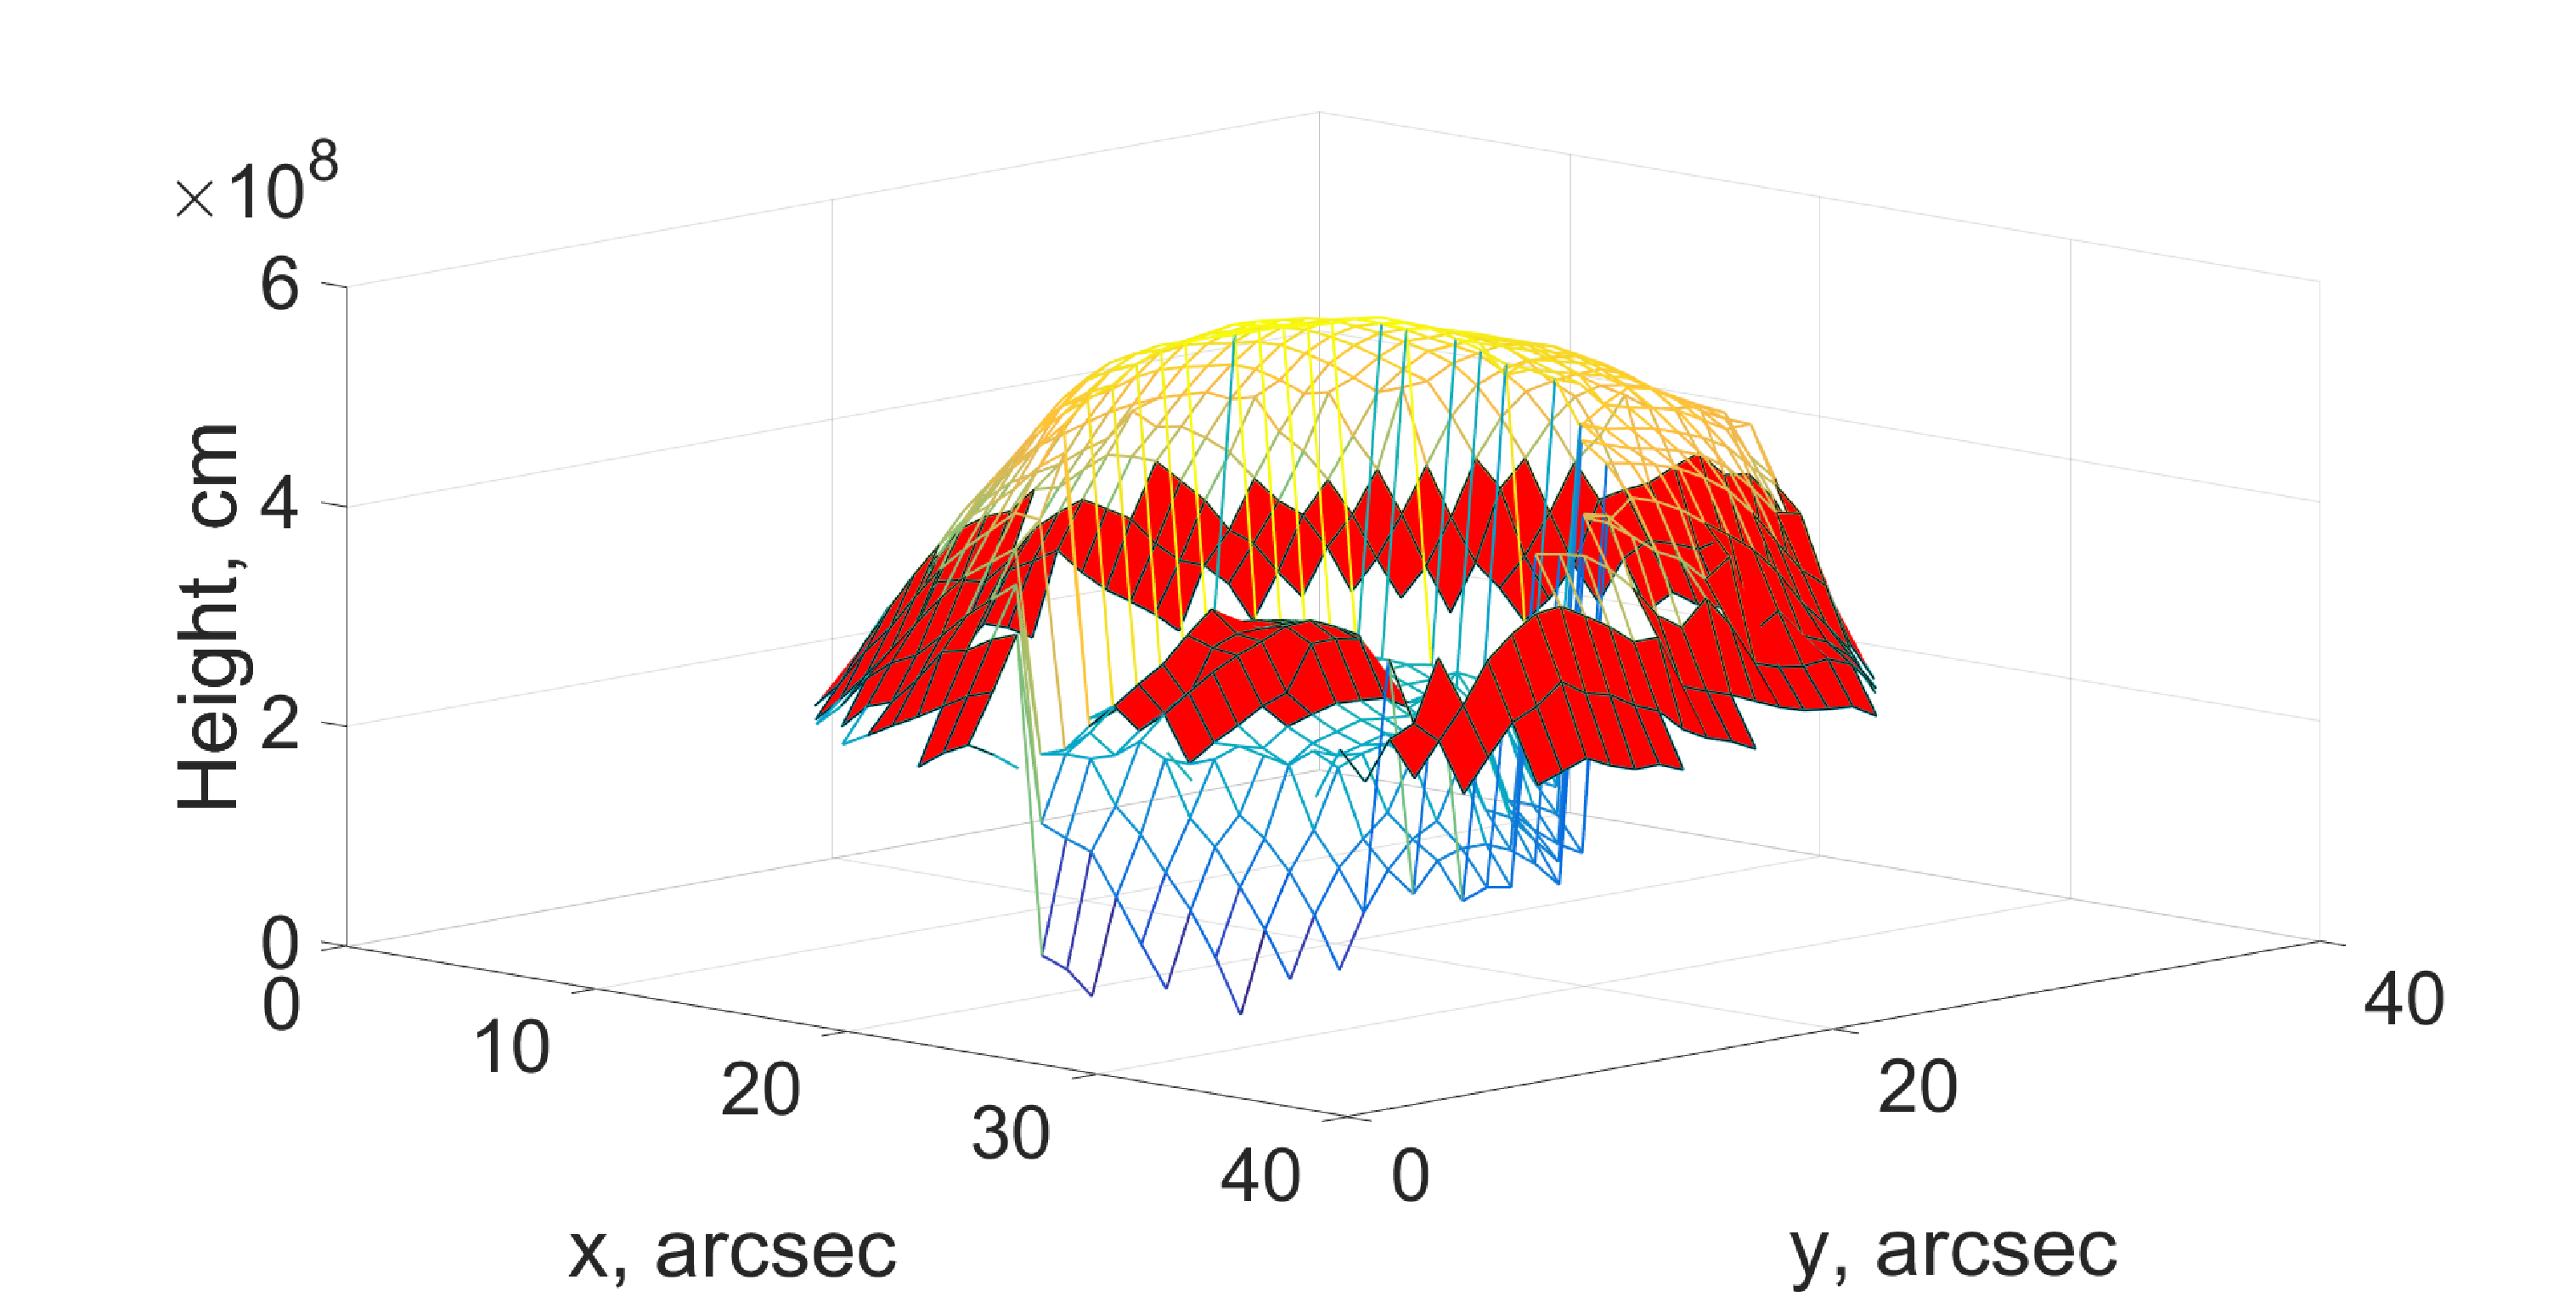
\includegraphics[width=1\linewidth]{images/Heights_tau_1.eps}
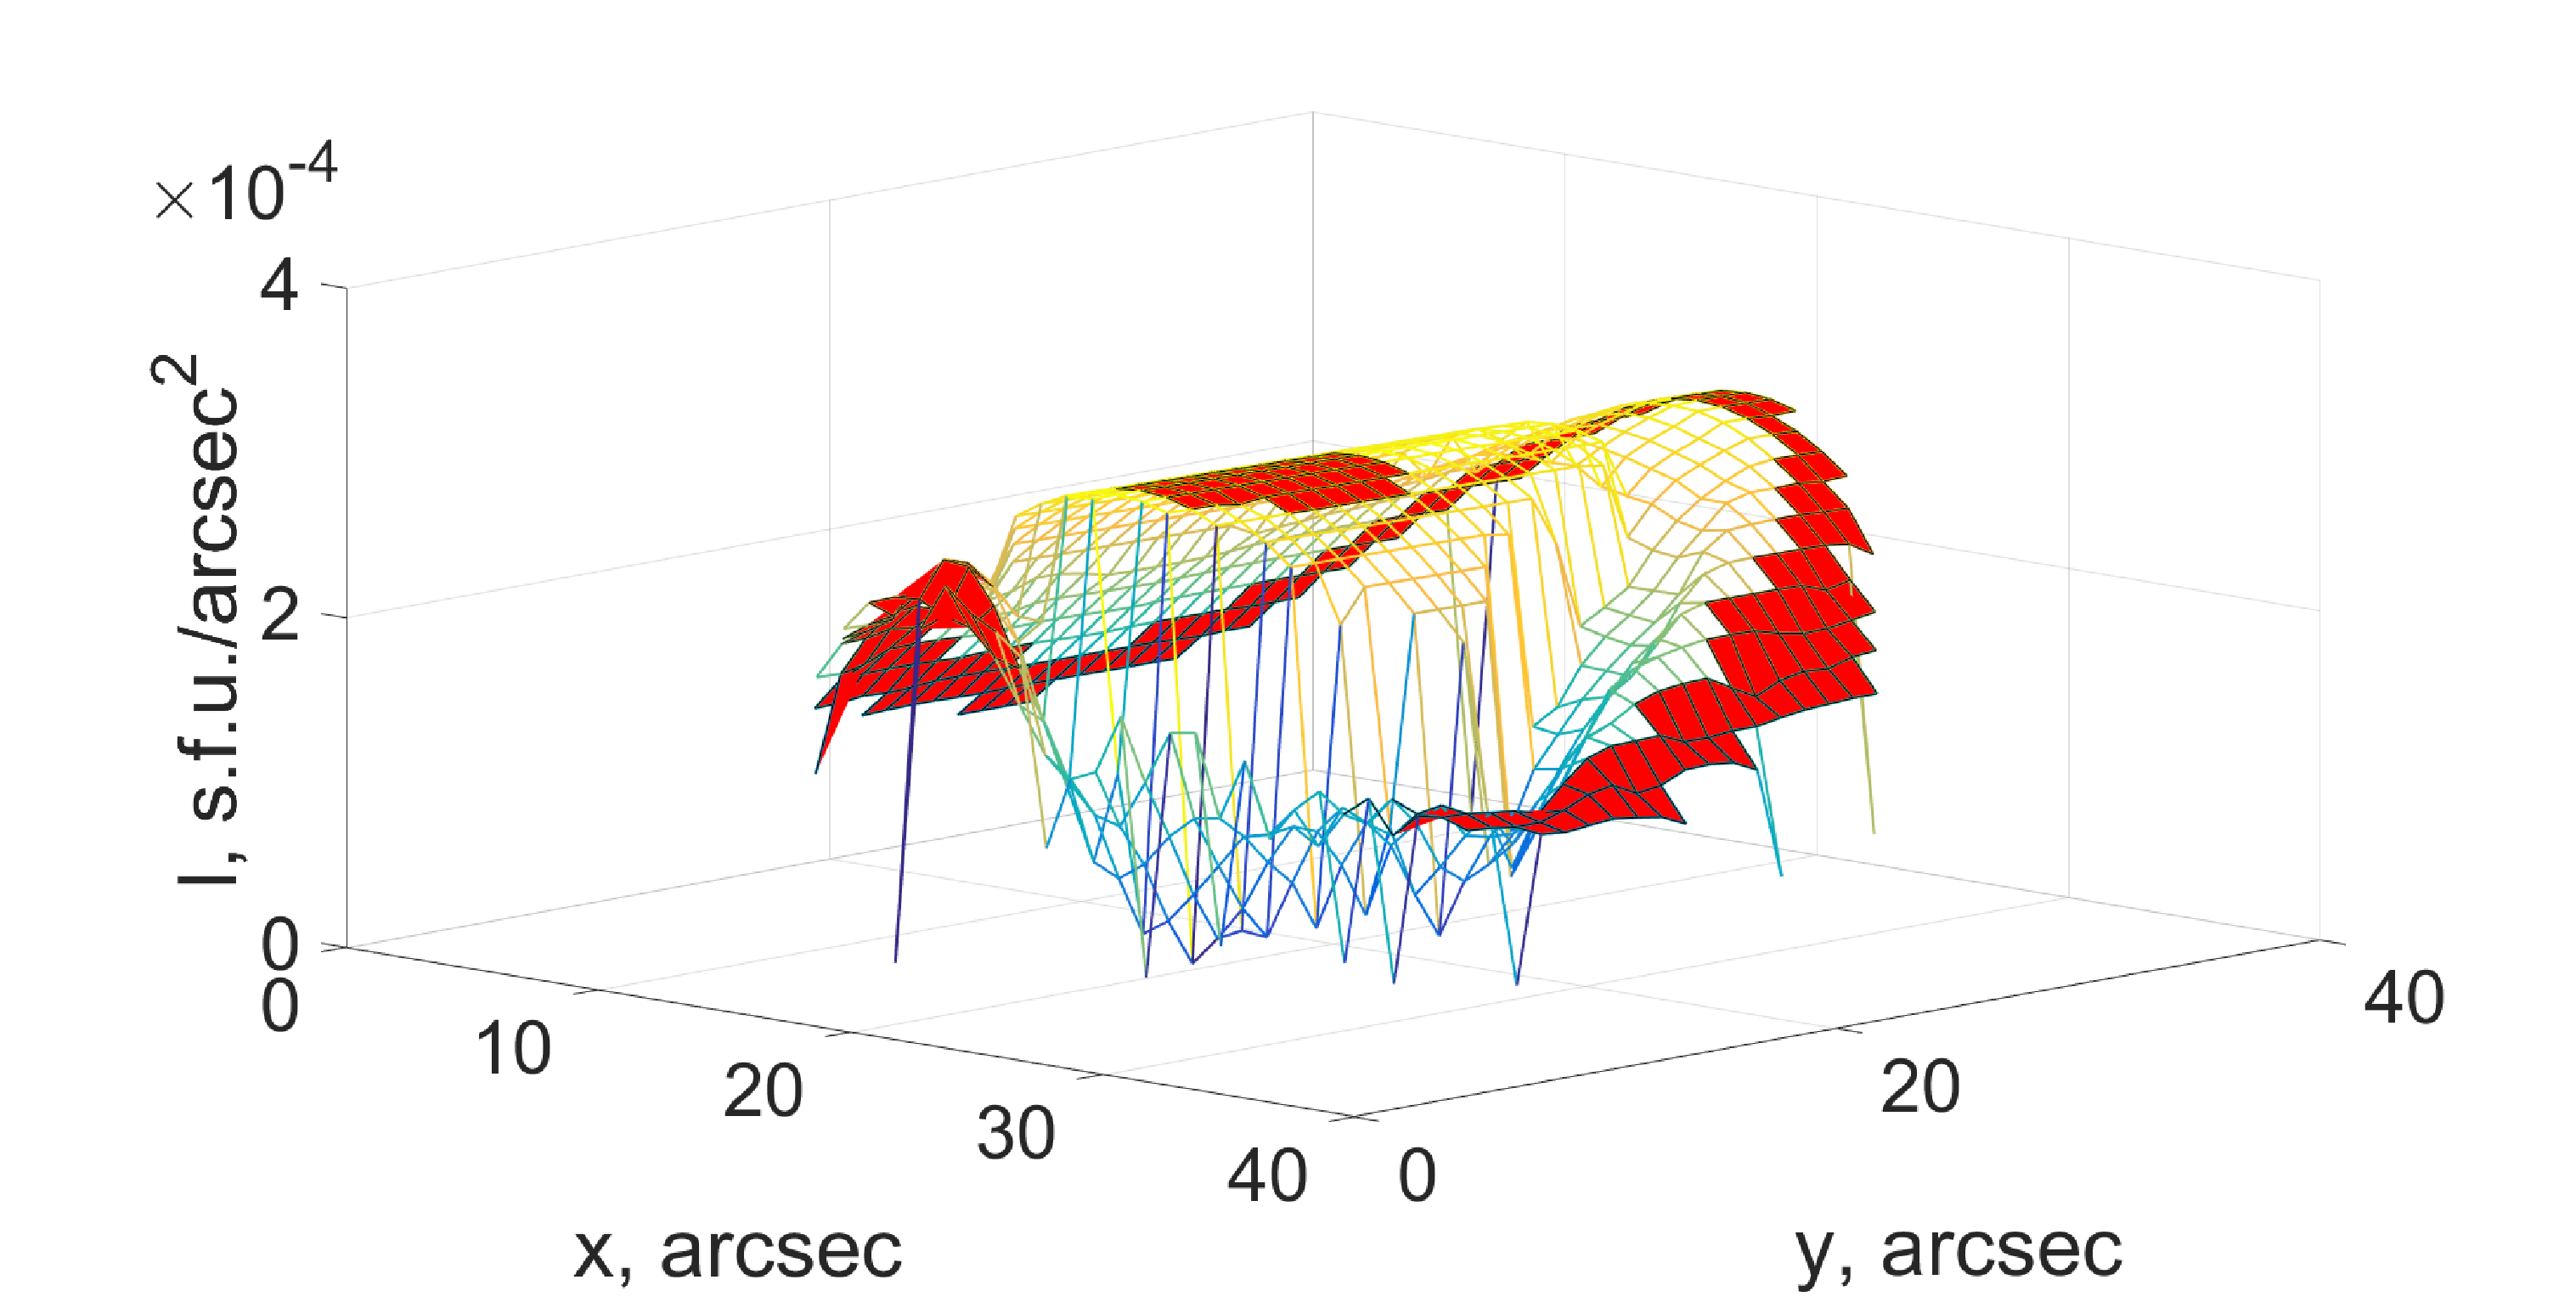
\includegraphics[width=1\linewidth]{images/Intensity_tau_1.eps}
\caption{Верхний рисунок: поверхности гироуровней 2-й и 3-й гармоник; 
красным выделены пиксели слоя $h_i$, на которых достигается $\tau \approx 1$. 
Нижний рисунок: поверхность интенсивности. 
Суммирование в уравнении (\ref{eq:summa_tau_1}) проводится по пикселям, выделенным красным.
}
\label{ris:pixels_tau_1}
\end{figure}


\begin{equation}
F_{\nu,p,i} = \sum_{x,y: \, \tau \approx 1} \, F_{\nu,p,i}(x, y),
\label{eq:summa_tau_1}
\end{equation}

где $x, y$ - координаты на сетке ${X, Y}$ (см. рис.~\ref{ris:pixels_tau_1}). Тогда полный модельный поток $F_{\nu,p}$ может быть получен суммированием по высотным слоям:

\begin{equation}
F_{\nu,p}^{\mathrm{model}} = \sum_{i=1}^M \, F_{\nu,p,i} + F_{\nu,p}^{\mathrm{thin}},
\label{eq:summa_by_layers}
\end{equation}

\begin{equation}
F_{\nu,p}^{\mathrm{thin}} = \sum_{x,y: \, \tau < 1} \, F_{\nu,p}^{} .
\end{equation}

$F_{\nu,p}^{\mathrm{thin}}$ представляет собой
%остаточный
вклад от оптически тонкой части атмосферы, который невозможно привязать к какому-то высотному слою.


%Модельный поток почти наверняка не будет совпадать с наблюдаемым,

Наша цель --- добиться максимально возможного совпадения расчетных ($F_{\nu,p}^{\mathrm{model}}$) и наблюдаемых ($F_{\nu,p}^{\mathrm{obs}}$) потоков, т.е. выполнения соотношения
\begin{equation}
F_{\nu,p}^{\mathrm{model}} = F_{\nu,p}^{\mathrm{obs}}, \qquad \forall \nu, p
\end{equation}
или, с учетом выражения (\ref{eq:summa_by_layers}),
\begin{equation}
\sum_{i=1}^M \, F_{\nu,p,i} = F_{\nu,p}^{\mathrm{obs}} - F_{\nu,p}^{\mathrm{thin}}. \qquad \forall \nu, p
\label{eq:equal_fluxes}
\end{equation}

Поскольку начальный температурно-высотный профиль задаётся произвольно, соответствующий ему модельный поток, вообще говоря, не согласуется с наблюдаемым спектром:
 некоторые высотные слои будут давать вклад меньший, чем реальный физический слой, некоторые больший. Нам  необходимо разработать механизм, позволяющий скорректировать вклад потоков с разных высотных слоев, корректируя температуры слоев.

Определим набор коэффициентов $\alpha_i$ ($i=1 \dots M$) для коррекции
температуры на  $k$-й итерации:

\as{
\begin{equation}
T_i^{(k+1)} = \alpha_i\, T_i^{(k)}.
\label{eq:TempCorrection}
\end{equation}
}

В условиях локального термодинамического равновесия (LTE) поток $F \sim T$, поэтому можем записать предыдущее соотношение как

\begin{equation}
F_{\nu,p,i}^{(k+1)} = \alpha_i\, F_{\nu,p,i}^{(k)}.
\label{eq:corr_coefs}
\end{equation}

%\begin{equation}
%F_{\nu}^{\mathrm{model}} = \sum_{i} \alpha_i\, F_{i,\nu} + %F_{\nu}^{\mathrm{thin}},
%\end{equation}

% где $F_{i,\nu}$ --- вклад $i$-го высотного слоя в модельный поток на частоте $\nu$, коэффициенты $\alpha_i$ являются корректирующими множителями, вводимыми на данной итерации алгоритма и отражающими относительное изменение температуры в соответствующих слоях, 

%Корректирующие множители $\alpha_i$ вводятся таким образом, что обновление температурного профиля на очередной итерации имеет вид
%\[
%T_i^{(n+1)} = \alpha_i \, T_i^{(n)} .
%\]

Уравнения (\ref{eq:equal_fluxes}), (\ref{eq:corr_coefs}) приводят нас к системе линейных уравнений для определения корректирующих коэффициентов:

\begin{equation}
\mathbf{F}\,\vec{\alpha} = \vec{f},
\label{eq:SLEBase}
\end{equation}

% где матрица $\mathbf{F}$ содержит вклад каждого высотного слоя в наблюдаемый поток на заданной частоте и в заданной поляризации, вектор $\vec{\alpha}$ состоит из искомых корректирующих множителей, а вектор $\vec{f}$ представляет собой разность между наблюдаемым и модельным потоками.

Матрица $\mathbf{F}$ имеет вид
\begin{equation}
\mathbf{F} =
\left(
\begin{matrix}
R^{(1)}_1 & R^{(2)}_1 & \hdots & R^{(M)}_1 \\
R^{(1)}_2 & R^{(2)}_2 & \hdots & R^{(M)}_2 \\
\hdots & \hdots & \ddots & \hdots \\
R^{(1)}_{N_R} & R^{(2)}_{N_R} & \hdots & R^{(M)}_{N_R} \\
L^{(1)}_1 & L^{(2)}_1 & \hdots & L^{(M)}_1 \\
L^{(1)}_2 & L^{(2)}_2 & \hdots & L^{(M)}_2 \\
\hdots & \hdots & \ddots & \hdots \\
L^{(1)}_{N_L} & L^{(2)}_{N_L} & \hdots & L^{(M)}_{N_L}
\end{matrix}
\right),
\end{equation}
где $R^{(j)}_k$ и $L^{(j)}_k$ --- вклад $i$-го слоя в модельный поток на $j$-й частоте в правой и левой круговых поляризациях соответственно.

Вектор корректирующих множителей имеет вид
\begin{equation}
\vec{\alpha} =
\left(
\begin{matrix}
\alpha_1 \\
\alpha_2 \\
\vdots \\
\alpha_M
\end{matrix}
\right),
\end{equation}
а вектор правой части определяется как
\begin{equation}
\vec{f} =
\left(
\begin{matrix}
R^{\mathrm{obs}}_{1} - R^{\mathrm{thin}}_{1} \\
R^{\mathrm{obs}}_{2} - R^{\mathrm{thin}}_{2} \\
\vdots \\
R^{\mathrm{obs}}_{N_R} - R^{\mathrm{thin}}_{N_R} \\
L^{\mathrm{obs}}_1 - L^{\mathrm{thin}}_1 \\
L^{\mathrm{obs}}_2 - L^{\mathrm{thin}}_2 \\
\vdots \\
L^{\mathrm{obs}}_{N_L} - L^{\mathrm{thin}}_{N_L}
\end{matrix}
\right).
\end{equation}

${N_R}, {N_L}$ --- количество наблюдаемых (и моделируемых) частот в правой и левой поляризации, соответственно.


%{\tk Здесь может быть уточнена форма регуляризующего условия и его реализация в матричной форме.}

% Система линейных уравнений с учётом регуляризации решается методом наименьших квадратов.


Для стабилизации решения и обеспечения его физической правдоподобности используется регуляризация в виде условия гладкости температурного профиля, требующего подавления резких вариаций температуры между соседними слоями:

\begin{equation}
\alpha_i T_i = \alpha_{i+1} T_{i+1} \qquad \forall\, i .
\end{equation}

Данное условие добавляется к системе линейных уравнений (\ref{eq:SLEBase}). В окончательной форме система будет иметь вид

\begin{equation}
\Theta \vec \alpha = \vec \phi, 
\end{equation}
где
\begin{equation}
\Theta = \left( 
\begin{matrix}
\textbf{F} \\
\textbf{T} \\
\end{matrix}
\right), \quad \vec \phi = \left( 
\begin{matrix}
\vec f \\
\vec 0 \\
\end{matrix}
\right),
\end{equation}

\textbf{T} --- двудиагональная матрица размера $(M-1) \times M$:

\begin{equation} \label{SLE_2diagT}
\textbf{T} =
\left( 
\begin{matrix}
T_1    & -T_2   &  0     & \hdots & 0         & 0      \\
0      &  T_2   & -T_3   & \hdots & 0         & 0      \\
\hdots & \hdots & \hdots & \ddots & \hdots    & \hdots \\
0      &  0     &  0     & \hdots & T_{M-1}   & -T_M   \\
\end{matrix}
\right).
\end{equation}

Такая расширенная система переопределена (т.к. имеет $M$ столбцов и $N_R+N_L+M-1$ строк), поэтому необходимо искать решение методом наименьших квадратов. Решение имеет вид

\begin{equation}
\vec \alpha = (\Theta' \textbf{W} \Theta)^{-1} \Theta' \textbf{W} \vec \phi
\label{eq:LMS}
\end{equation}

где $\mathbf{W}$ --- весовая матрица. В простейшем случае это просто единичная матрица. Но если у нас есть априорные оценки значимости отдельных уравнений, мы можем понижать вес отдельных уравнений (например, вес может быть меньше для более зашумленных частот и т.д.).

%, в которой меньшие веса назначаются частотам с меньшим вкладом в формирование наблюдаемого излучения, а вектор
%\begin{equation}
%\vec{v} = \vec{F}^{\,\mathrm{obs}} - \vec{F}^{\,\mathrm{model}}
%\end{equation}
%представляет собой разность между наблюдаемыми и модельными потоками.
%{\tk Здесь может быть уточнён вид весовой матрицы и процедура решения.}

Итерационный процесс восстановления температурно-высотного профиля строится следующим образом:
\begin{enumerate}
  \label{list:iterations}
  \item Задаётся начальное приближение к температурно-высотному профилю $\{T_i^{(0)}\}$.
  
  \item На $k$-й итерации по текущему температурному профилю $\{T_i^{(k)}\}$ рассчитывается модельный микроволновый поток $F_{\nu, p}^{\mathrm{model}}$ и его составляющие $F_{\nu,p,i}^{\mathrm{model}}$, $F_{\nu,p}^{\mathrm{thin}}$ на всех рассматриваемых частотах и в обеих круговых поляризациях (уравнения (\ref{eq:summa_tau_1}),(\ref{eq:summa_by_layers})).

  \item На основе решения уравнения (\ref{eq:LMS}) определяется вектор корректирующих множителей $\{\alpha_i^{(k)}\}$.
  
  \item Температурный профиль для итерации $k+1$ обновляется согласно соотношению (\ref{eq:TempCorrection}):
  \begin{equation*}
  T_i^{(k+1)} = \alpha_i^{(k)}\, T_i^{(k)} .
  \end{equation*}
  
  \item  Итерации выполняются до стабилизации невязки между модельным и наблюдаемым спектрами.
Критерием останова является изменение невязки ниже заданного порога в течение нескольких последовательных шагов.

\end{enumerate}

Сходимость алгоритма, как правило, достигается за $10$--$30$ итераций.

%{\tk Здесь может быть уточнён используемый критерий невязки и численные параметры останова.}

% конец  нового  враианта

\section{ТЕСТИРОВАНИЕ НА ДИПОЛЬНОЙ МОДЕЛИ}
%----------------------------------------------------------------------------------------------------------------
\subsection{Описание модели}
%{\todo
%\begin{itemize}
%  \item Магнитное поле: вертикальный диполь, погружённый на фиксированную глубину.
%  \item Температурно-высотный профиль: хромосфера, переходная область, корона.
%\end{itemize}
%}


% новый  вариант начало


Для первичной верификации итерационного метода используется упрощённая модель солнечного пятна с заданной магнитной конфигурацией и температурно-высотным профилем атмосферы. Применение модельных данных позволяет проверить корректность работы алгоритма в контролируемых условиях, при известном истинном температурном распределении.

Численное моделирование микроволнового излучения выполнялось с использованием программного пакета расчёта гирорезонансного излучения, разработанного в \citep{Stupishin2018}.


Магнитное поле в модели задаётся в виде вертикального магнитного диполя, расположенного в центре солнечного диска и погружённого под фотосферу на глубину
%$h_{\mathrm d} = 1.6 \times 10^{4}$~км.
 $h_d = 16\,\mathrm{Mm}$.

%\asq{Может, везде систематически писать Мм} 

Такое приближение обеспечивает реалистичное убывание напряжённости магнитного поля с высотой и воспроизводит характерную магнитную конфигурацию одиночных солнечных пятен \citep{Lites1990,Zlotnik1996, Brosius1989}.

Максимальная напряжённость магнитного поля в основании пятна $B_{\max}$ \as{полагалась равной 3000~Гс --- типичному значению для солнечного пятна.}
 Дополнительно варьируется пространственное разрешение вычислительной сетки радиокарты, что позволяет оценить влияние численных параметров на результаты моделирования.   


Температурно-высотный профиль атмосферы задаётся в виде трёх характерных зон:
холодной плотной хромосферы до высоты $h \approx 1.5\,\mathrm{Mm}$ с температурой
$T \simeq 10^{4}$~К,
переходной области на высотах $1.5$\,--\,$1.8\,\mathrm{Mm}$ с резким ростом температуры, \as{переходящей к корональным значениям $T \simeq 1 \times 10^{6}$~К,
и горячей разреженной короны (до $2.5 \times 10^{6}$~К) при $h > 1.8\,\mathrm{Mm}$.}


Высотное распределение электронной концентрации $N(h)$ задаётся барометрическим законом (\ref{barometric}), исходя из заданного значения плотности в основании короны и  характерного масштаба изменения плотности с высотой.



\subsection{Генерация модельных данных}
%{\todo
%\begin{itemize}
%  \item Радиокарта по расчётному излучению.
%  \item Свертка с диаграммой направленности РАТАН-600.
%  \item Получение одномерного скана и спектра.
%\end{itemize}
%}


\begin{figure}
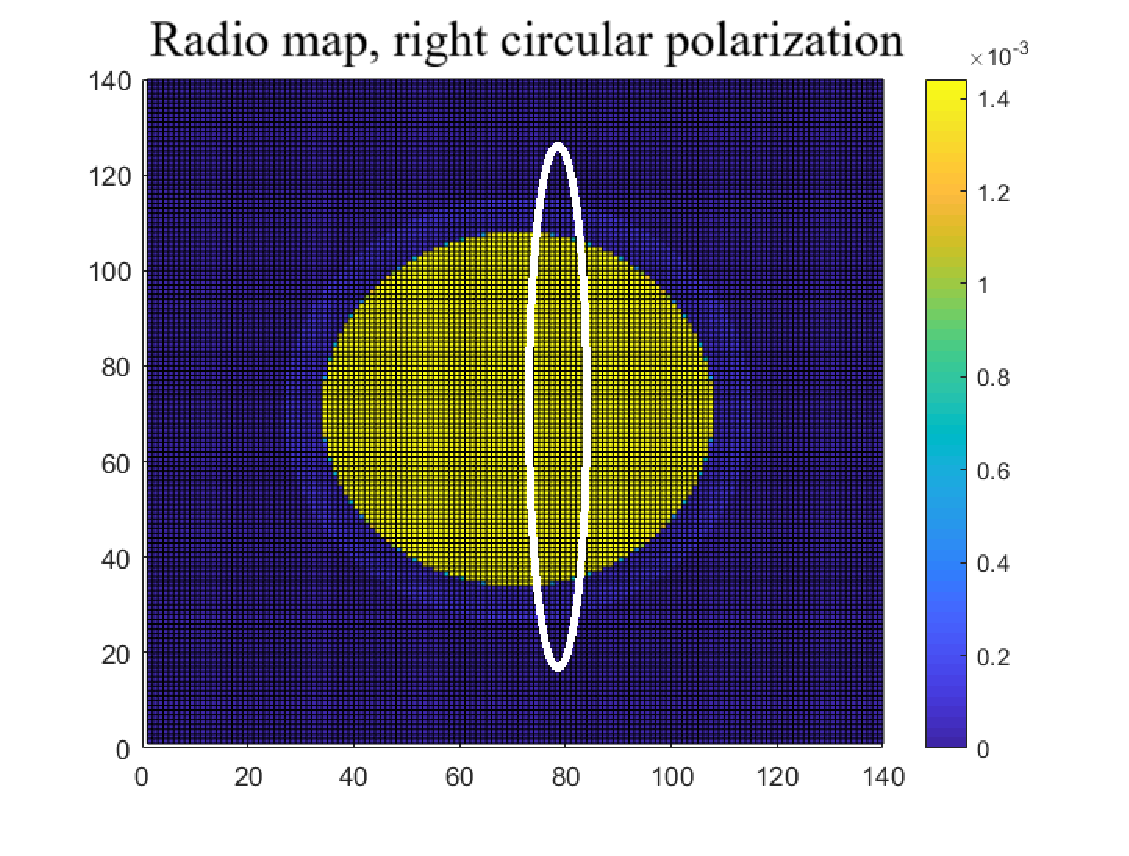
\includegraphics[width=0.8\linewidth]{images/Radiomap_R.eps}
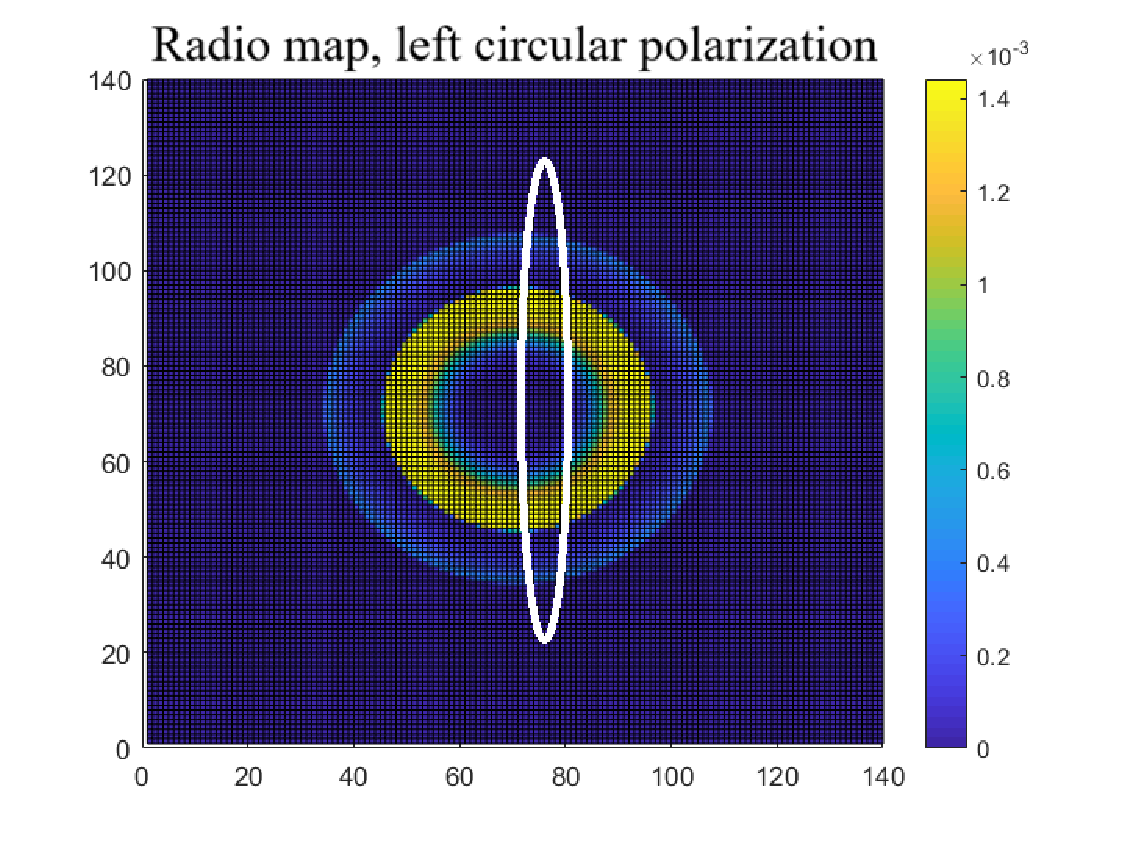
\includegraphics[width=0.8\linewidth]{images/Radiomap_L.eps}
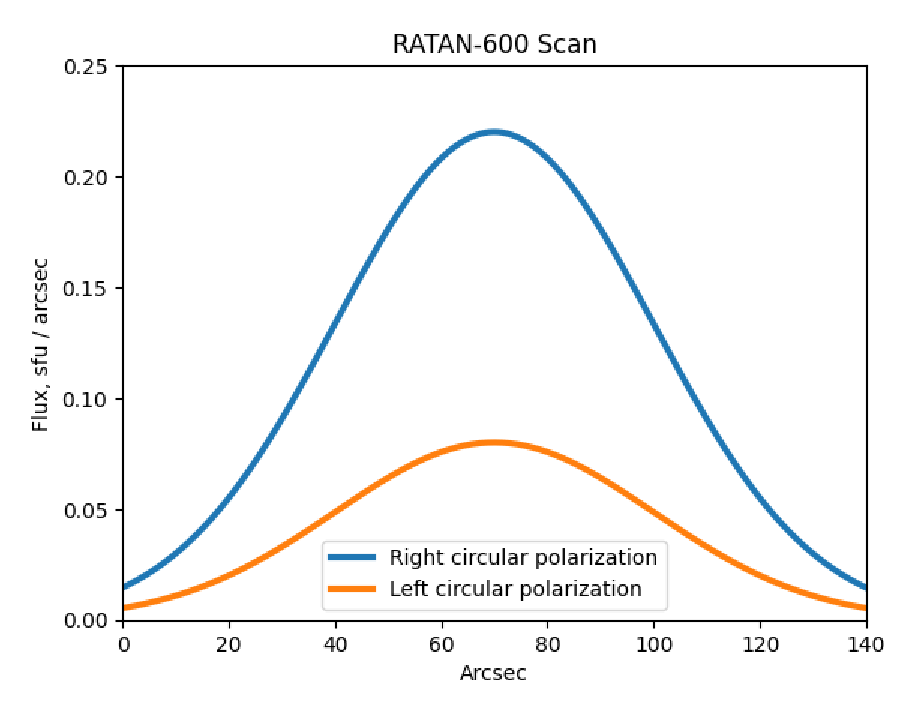
\includegraphics[width=0.7\linewidth]{images/cut_en.eps}
\caption{Сверху: расчётные радиокарты активной области для дипольной модели магнитного поля
($B_{\max}=3000$~Гс, $f=8$~ГГц) в правой и левой круговых поляризациях. Снизу: одномерные сканы, полученные в результате свёртки радиокарт с ДНА РАТАН-600.}
\label{ris:Radomap_scan}
\end{figure}

На основе заданной магнитной конфигурации и температурно-высотного профиля выполняется численное моделирование микроволнового излучения активной области. Для каждой частоты и каждой круговой поляризации рассчитываются радиокарты яркостной температуры с учётом гирорезонансного механизма излучения. Далее радиокарты свёртываются с диаграммой направленности РАТАН-600, что позволяет получить одномерные сканы, аналогичные реальным наблюдениям (рис.~\ref{ris:Radomap_scan}).

Из сканов извлекаются значения максимального потока на каждой частоте; их совокупность формирует модельный микроволновый спектр в правой и левой круговых поляризациях. Этот спектр используется как тестовый вход для итерационного алгоритма восстановления температурно-высотного профиля.

Тестирование проводится при различных начальных приближениях, включая существенно смещённые профили (например, с искусственно завышенной высотой переходной области), что позволяет оценить устойчивость и сходимость метода.

%-------------------------------------------------------
\subsection{Результаты тестов}
%{\todo
%\begin{itemize}
%  \item Сходимость к известному температурному профилю.
%  \item Устойчивость к начальным условиям.
%  \item Чувствительность к аддитивному и %мультипликативному шуму.
%\end{itemize}
%}

\begin{figure*}
%\includegraphics[width=1\linewidth]{images/Test.eps}
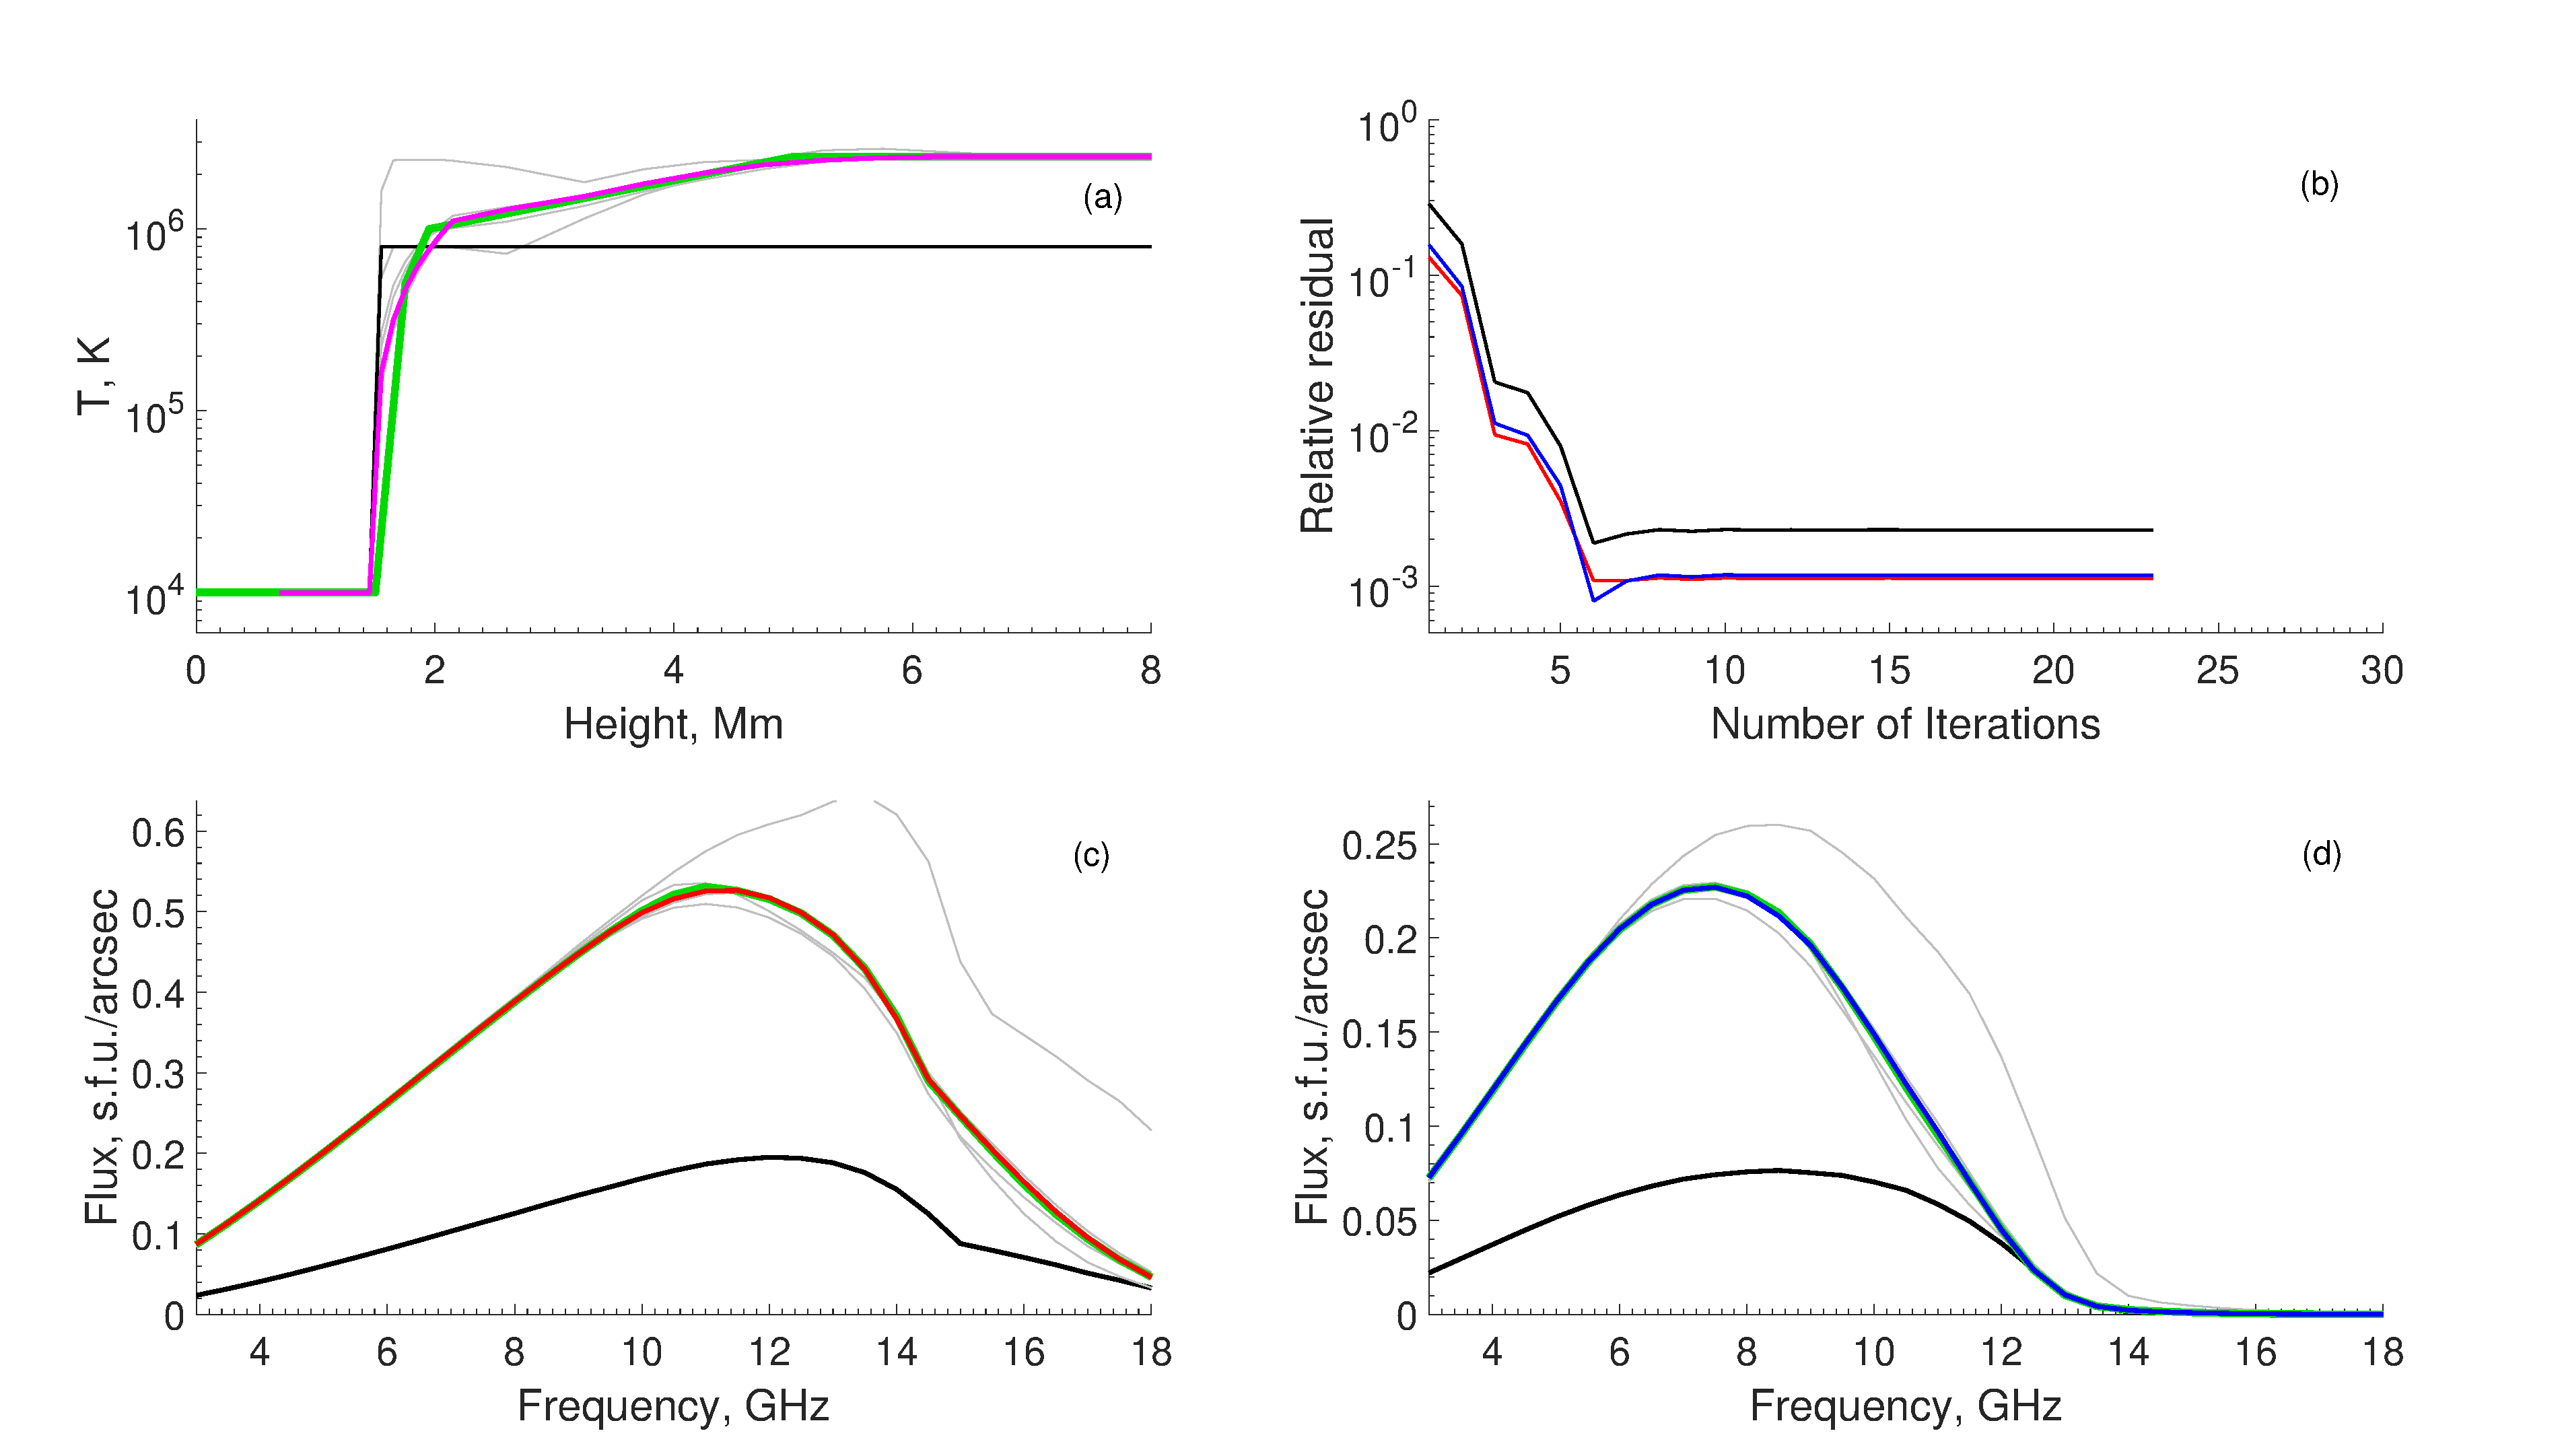
\includegraphics[width=1\linewidth]{images/Test_new.eps}
%\includegraphics[width=1\linewidth]{images/Testt.eps}
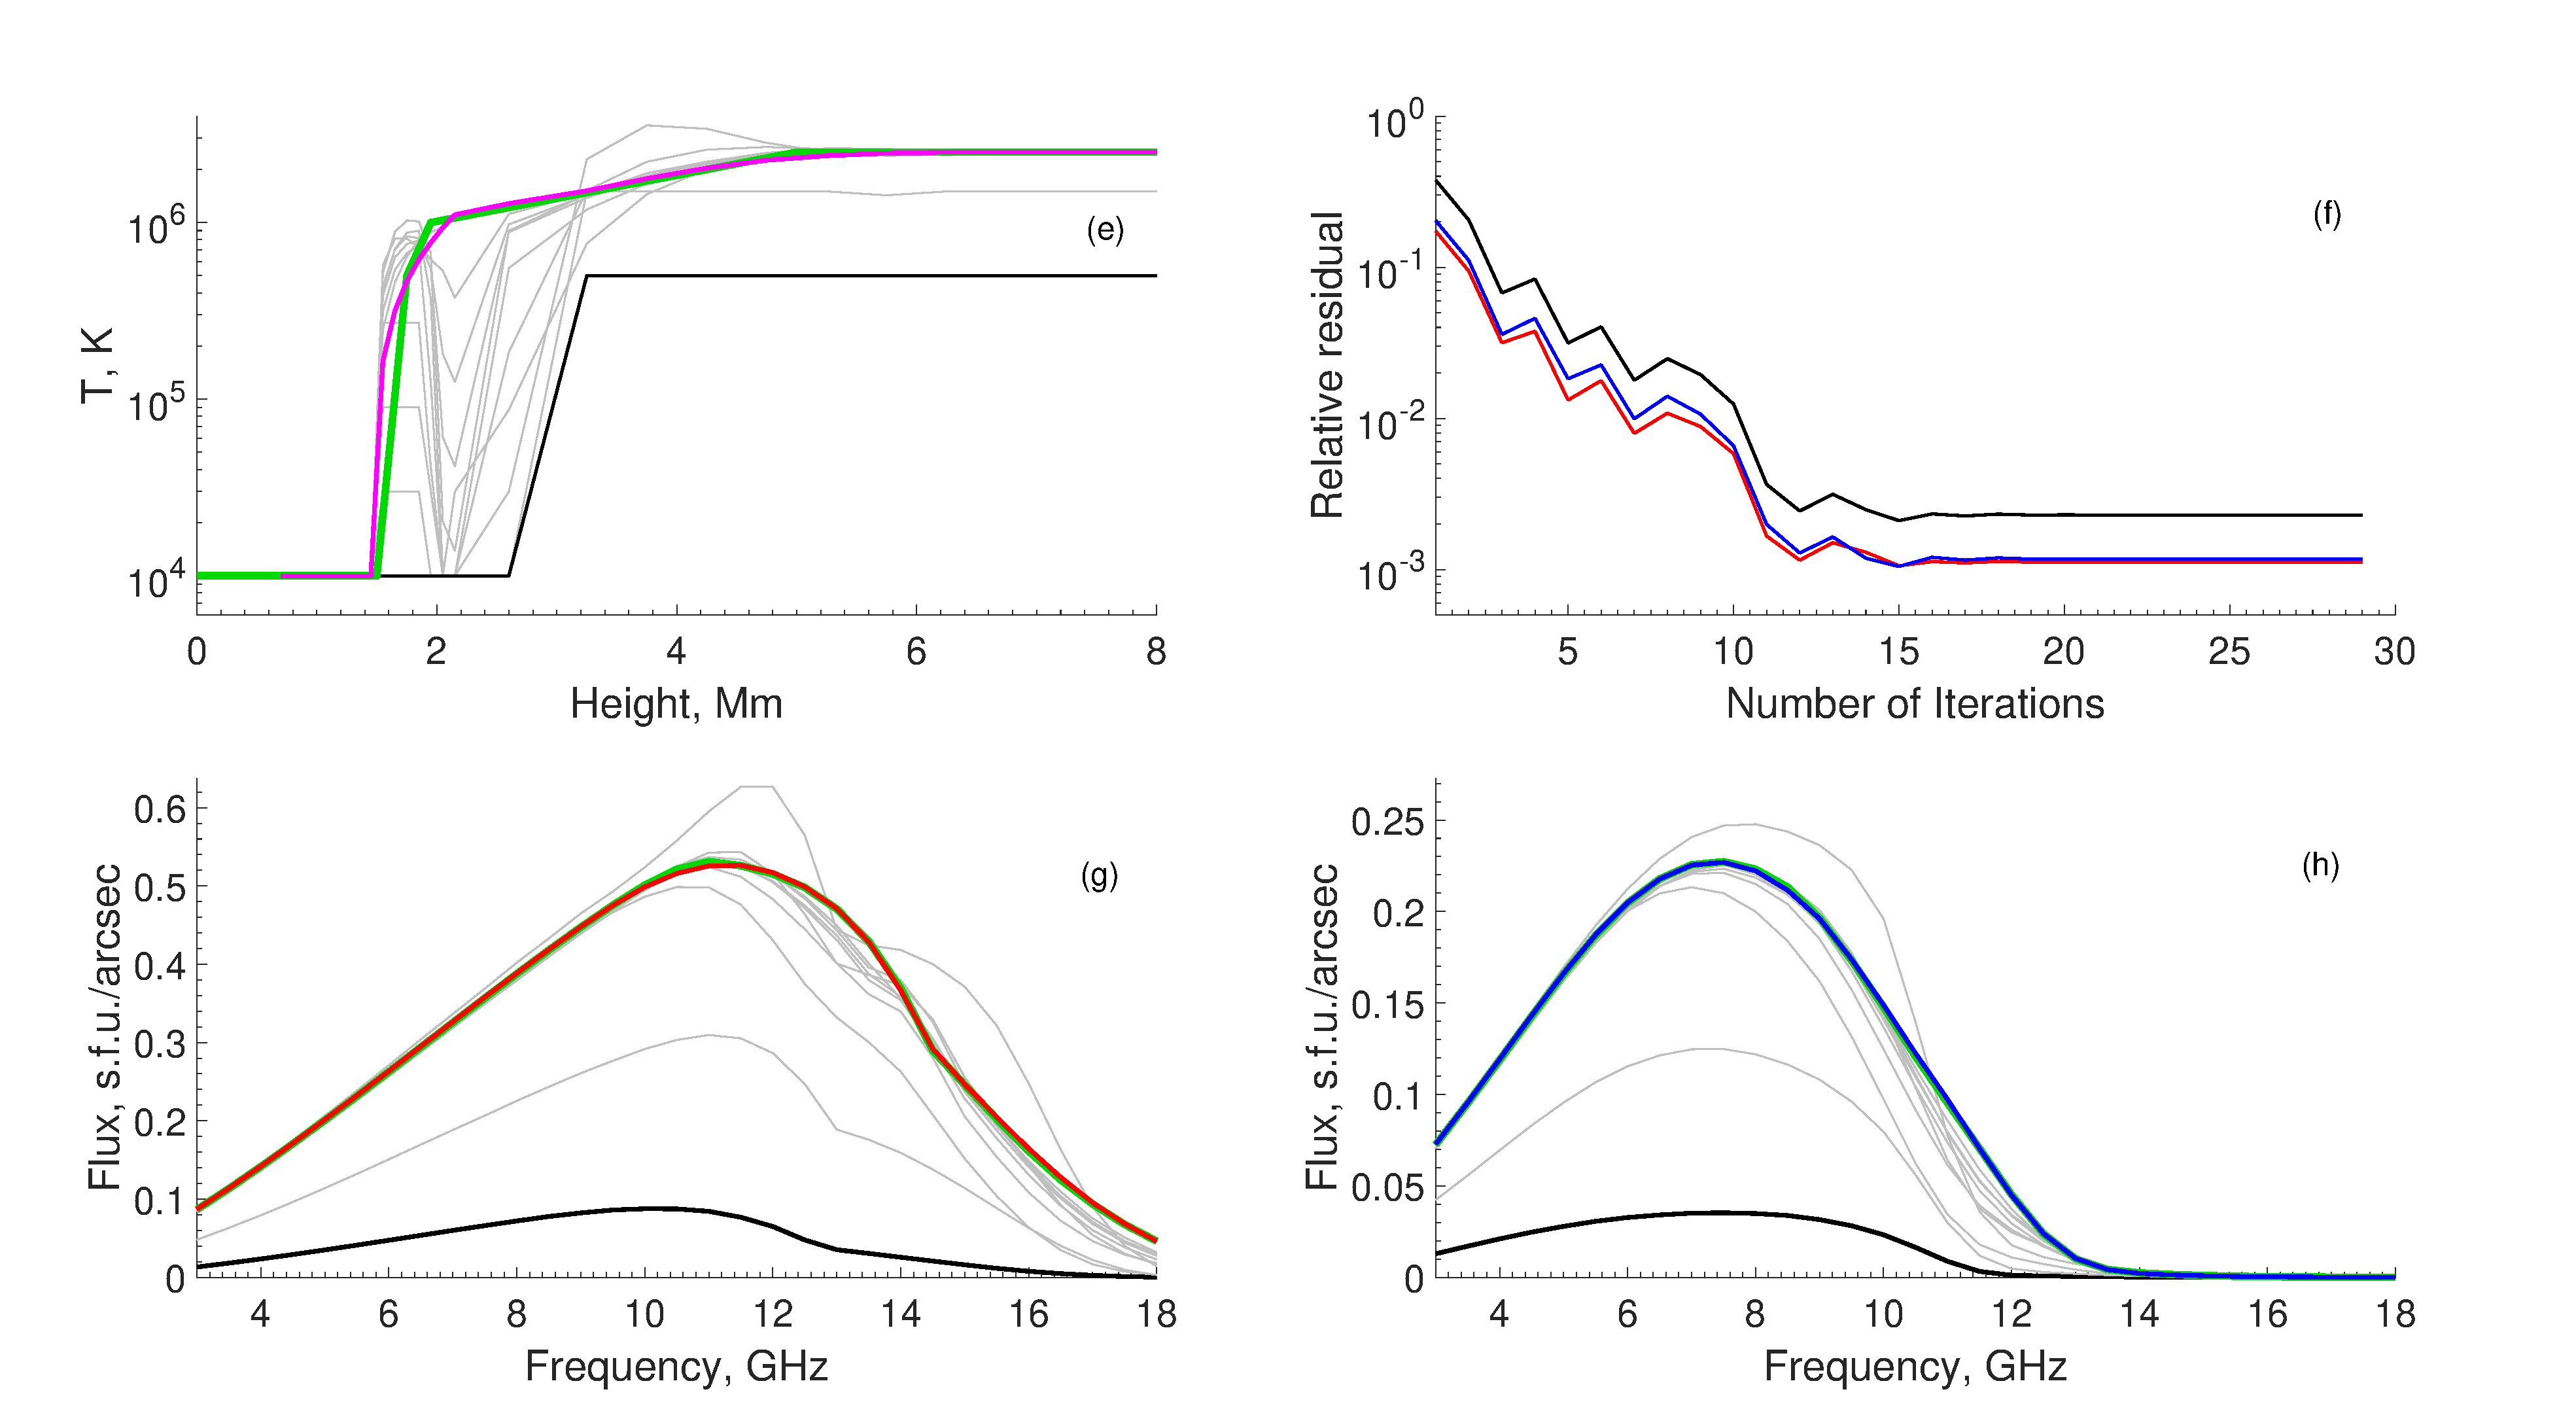
\includegraphics[width=1\linewidth]{images/Testt_new.eps}
\caption{\as{Результаты тестирования итерационного алгоритма восстановления температурно-высотного профиля
для дипольной модели активной области.
В верхней части (a,b,c,d) показан результат для начального температурного профиля, близкого к модельному,
в нижней (e,f,g,h) --- для начального профиля с искусственно завышенной высотой переходной области. 
В каждом случае приведены температурно-высотный профиль (a,e), зависимость невязки от номера итерации (b,f),
а также спектры микроволнового излучения в правой (c,g) и левой(d,h) круговых поляризациях.}}
\label{fig:Test}
\end{figure*}

Результаты тестирования алгоритма представлены на рис.~\ref{fig:Test}. Верхний блок соответствует случаю начального профиля, близкого к модельному, нижний --- существенно смещённому начальному приближению с завышенной высотой переходной области.

На панелях с температурно-высотными профилями зелёной кривой показано истинное распределение температуры, чёрной --- начальное приближение, фуксиновой --- восстановленный профиль после завершения итераций. Серые кривые отображают промежуточные итерации и иллюстрируют траекторию сходимости алгоритма.

Графики  относительной невязки демонстрируют уменьшение ошибки по мере итераций. Красная и синяя кривые соответствуют невязке в правой и левой круговых поляризациях соответственно, чёрная кривая --- их суммарной невязке. В обоих тестах наблюдается устойчивое снижение ошибки; в случае близкого начального профиля сходимость достигается за меньшее число шагов, тогда как при существенно смещённом начальном приближении требуется больше итераций, однако конечный уровень невязки также уменьшается до
\as{$\sim$\,0.2\,--\,0.3\,\%.}


На панелях со спектрами зелёные кривые соответствуют модельным (истинным) спектрам, красная и синяя --- восстановленным спектрам в правой и левой круговых поляризациях соответственно. Серые спектры отражают промежуточные итерации и демонстрируют постепенное приближение к модельному распределению.

Таким образом, алгоритм воспроизводит заданный температурно-высотный профиль даже при существенно искажённом начальном приближении, сохраняя устойчивость и контролируемую сходимость.



\subsection{Чувствительность метода к шуму во входных спектрах}
\label{sec:noise_sensitivity}


\begin{figure*}[t]
  \centering
  \begin{tabular}{cc}
    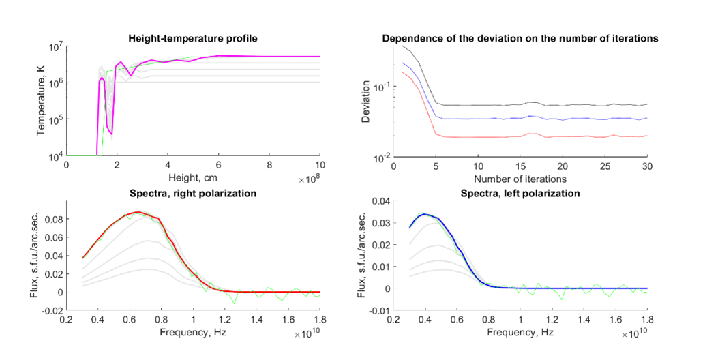
\includegraphics[width=0.48\textwidth]{images/noise_A5.eps} &
    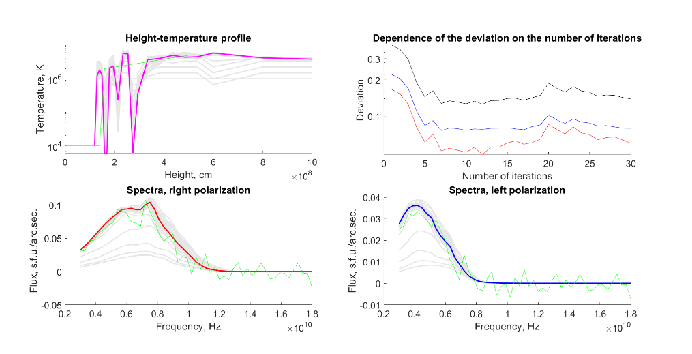
\includegraphics[width=0.48\textwidth]{images/noise_A10.eps}
  \end{tabular}
  \caption{
  Тестирование чувствительности итерационного метода к аддитивному шуму
  во входных спектрах.
  Показаны эталонный и восстановленный температурно-высотные профили,
  а также качество воспроизведения спектров в правой и левой круговых
  поляризациях.
  (a) аддитивный шум с уровнем $5\%$;
  (b) аддитивный шум с уровнем $10\%$.
  }
  \label{fig:noise_add}
\end{figure*}

\begin{figure*}[t]
  \centering
  \begin{tabular}{cc}
    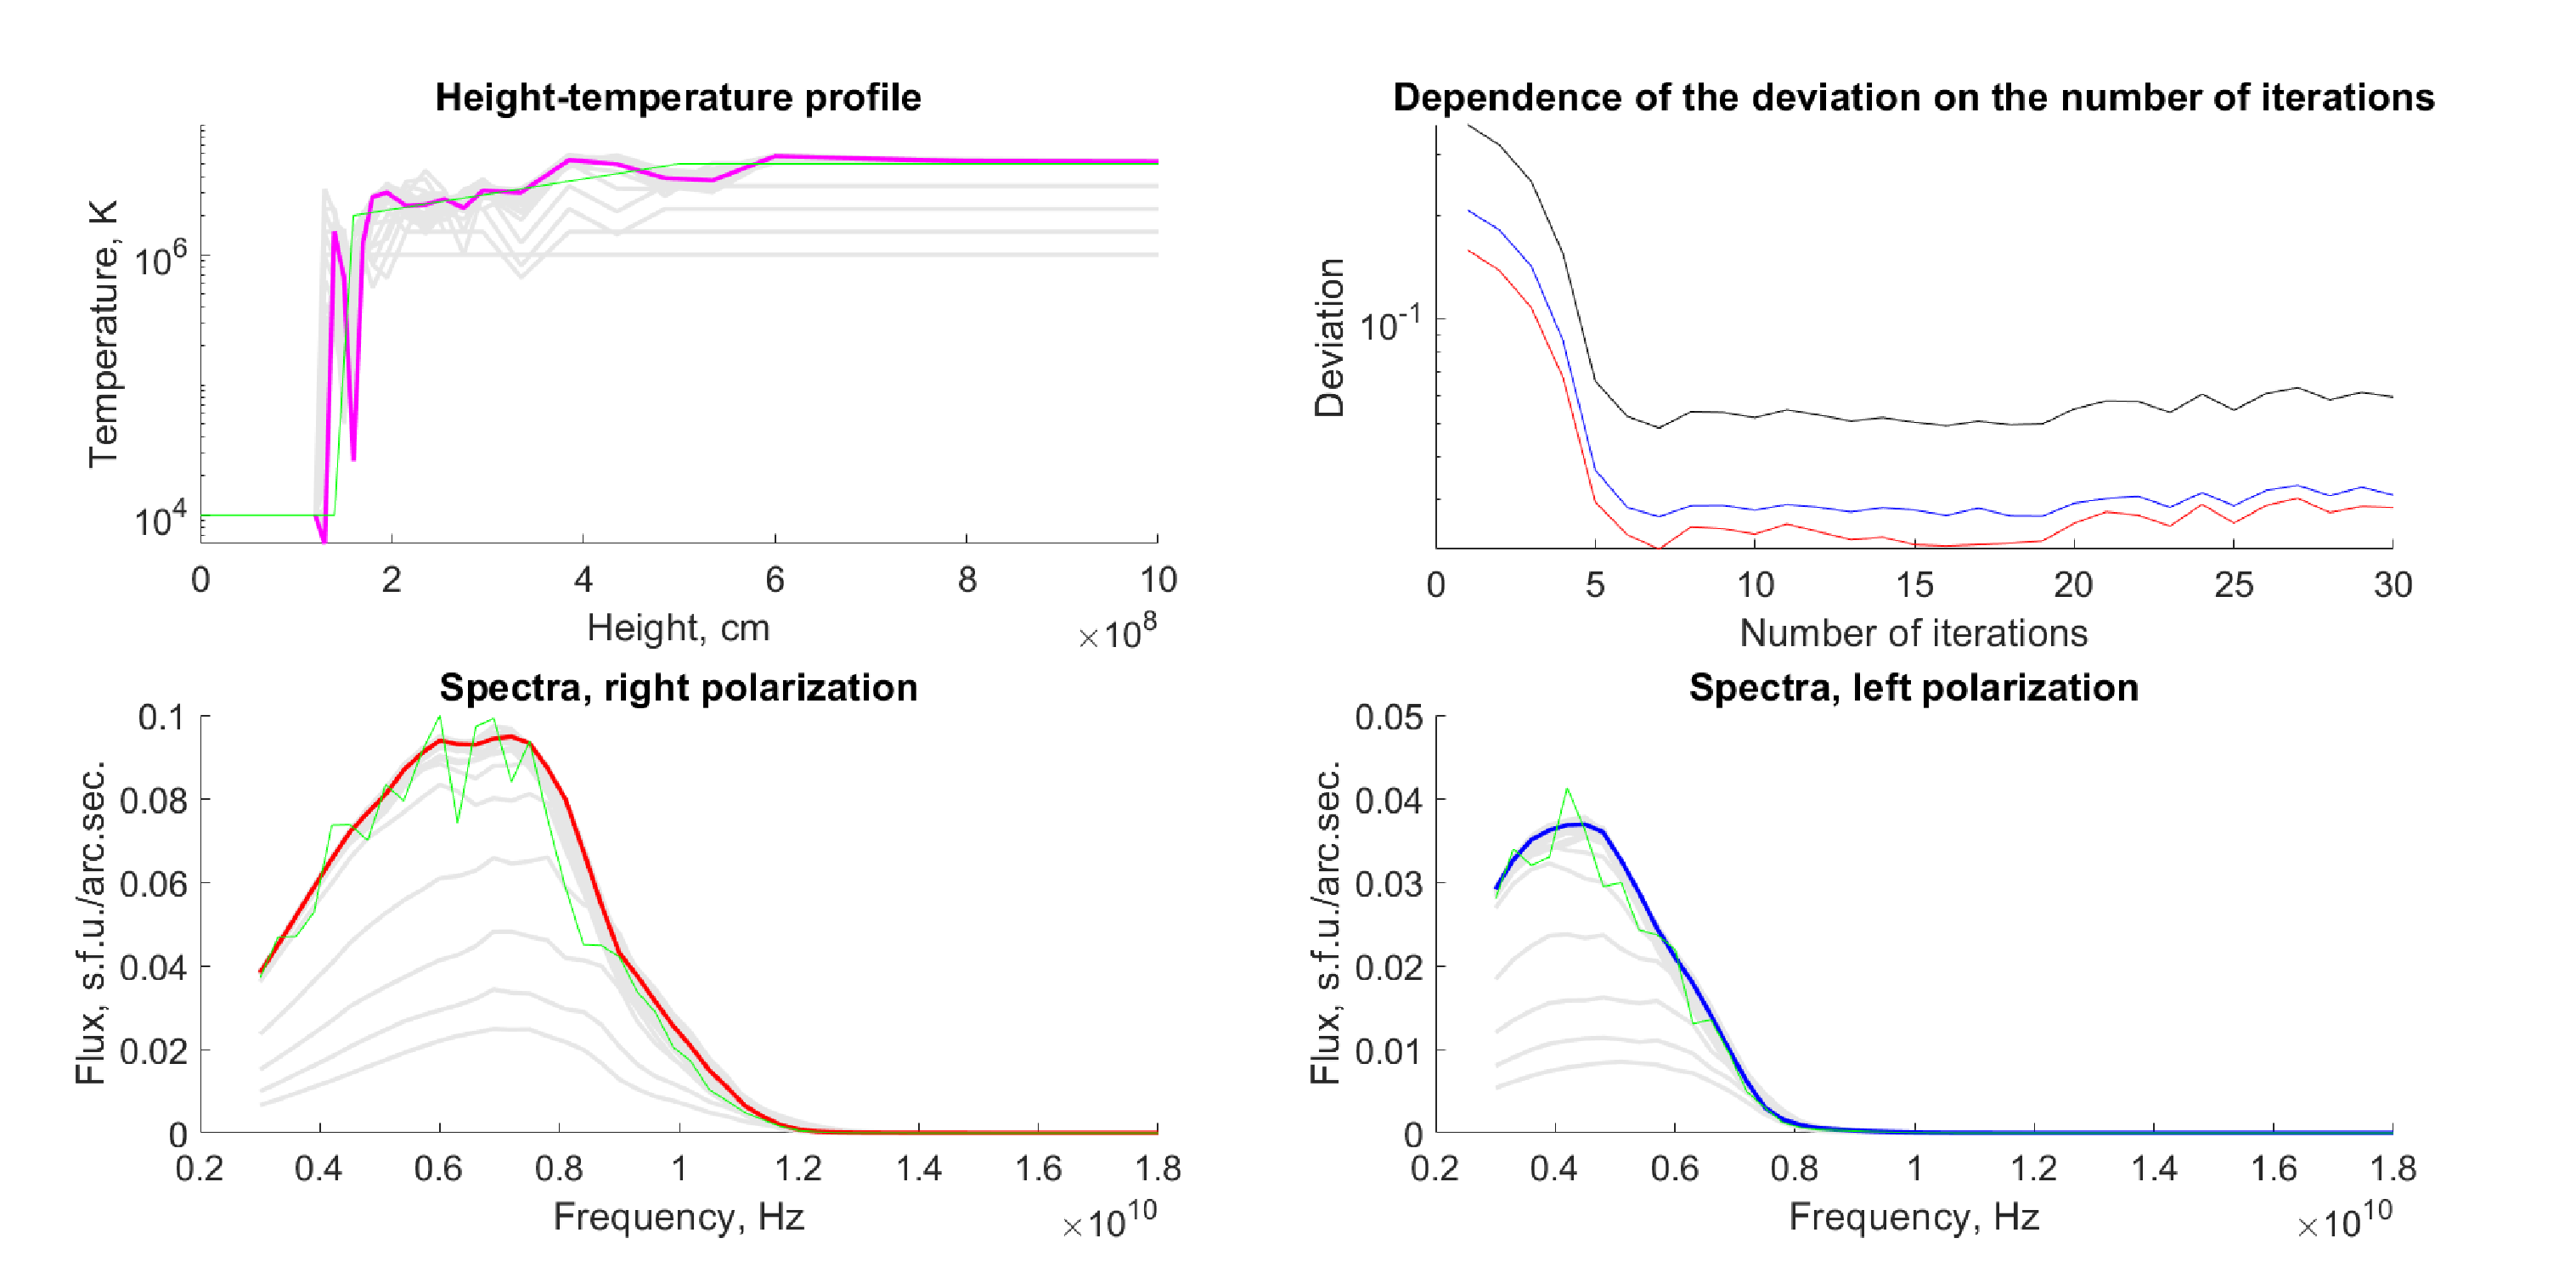
\includegraphics[width=0.48\textwidth]{images/noise_M10.eps} &
    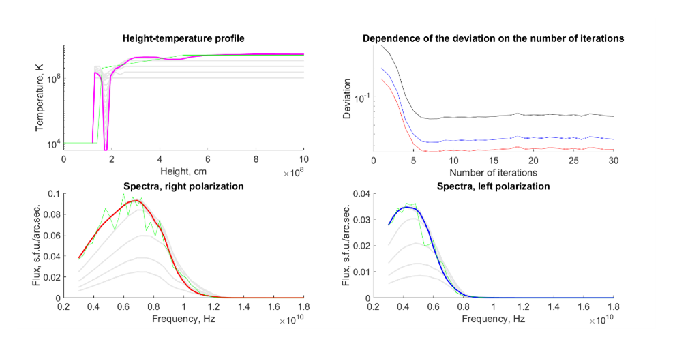
\includegraphics[width=0.48\textwidth]{images/noiseM10W10.eps}
  \end{tabular}
  \caption{
  Тестирование устойчивости итерационного метода к мультипликативному шуму
  и влияние усиления регуляризации.
  Показаны эталонный и восстановленный температурно-высотные профили,
  а также воспроизведение спектров в правой и левой круговых поляризациях.
  (a) мультипликативный шум с уровнем $10\%$;
  (b) тот же уровень шума при увеличении весов регуляризующих
  (температурных) уравнений в 100  раз.
  }
  \label{fig:noise_mult_reg}
\end{figure*}



\label{sec:noise}

Для оценки устойчивости метода к искажениям входных спектров
к эталонному модельному спектру добавлялся искусственный шум
заданного типа и уровня, после чего температурно-высотный профиль
восстанавливался тем же алгоритмом.

Рассматривались два типа ошибок: аддитивные
(шумы приёмной системы и фоновые флуктуации)
и мультипликативные (ошибки калибровки и нестабильность усиления).
Аддитивный шум задавался как
\as{
\[
F_i' = F_i + \xi_i\, \sigma\, F_{\max},
\]
а мультипликативный ---
\[
F_i' = F_i (1 + \xi_i\, \sigma),
\]
}
где $\sigma$ --- относительный уровень шума,
$\xi_i \in [-1,1]$ --- случайная величина.

При малом зашумлении ($\sigma=1\%$, не показано)
восстановленный профиль практически совпадает с эталонным;
различия ограничиваются слабыми вариациями в области переходной зоны.
Для аддитивного шума при $\sigma=5\%$
становятся заметны искажения положения и крутизны переходной области,
тогда как корональная часть профиля остаётся устойчивой.
При $\sigma=10\%$ переходная зона становится основным источником
неопределённости; вклад шума становится доминирующим фактором,
ограничивающим точность реконструкции переходной области
(рис.~\ref{fig:noise_add}).

В случае мультипликативного шума восстановление оказывается более устойчивым.
Даже при $\sigma=10\%$ форма профиля в целом сохраняется,
а искажения переходной зоны выражены слабее
(рис.~\ref{fig:noise_mult_reg}a).
Это связано с тем, что мультипликативные ошибки
сохраняют относительную форму спектра,
тогда как аддитивный шум вносит частотно-независимую добавку
по амплитуде и сильнее искажает спектральную структуру сигнала.

При высоком уровне шума устойчивость восстановления
достигается за счёт усиления регуляризации.
Увеличение весов температурных уравнений приводит к сглаживанию
восстановленного профиля и подавлению нефизических осцилляций,
прежде всего в переходной зоне, однако сопровождается ростом
спектральной невязки, что отражает компромисс между гладкостью решения
и точностью воспроизведения зашумлённых данных
(рис.~\ref{fig:noise_mult_reg}b).
Приведённый на рисунке пример относится к случаю мультипликативного шума,
однако аналогичный результат получен и для аддитивного шума
при том же уровне $\sigma = 10\%$ при увеличении
весов регуляризующих уравнений в 100 раз.

Основные выводы тестирования состоят в том, что метод сохраняет
работоспособность при умеренном зашумлении входных спектров;
наиболее чувствительной областью восстановления остаётся переходная зона;
мультипликативный шум влияет на результат слабее, чем аддитивный
при сопоставимом уровне, а усиление регуляризации позволяет
стабилизировать решение при сильном шуме ценой увеличения невязки.



\section{ ПРИМЕНЕНИЕ МЕТОДА К НАБЛЮДЕНИЯМ АКТИВНОЙ ОБЛАСТИ NOAA 11312}


\begin{figure*}
	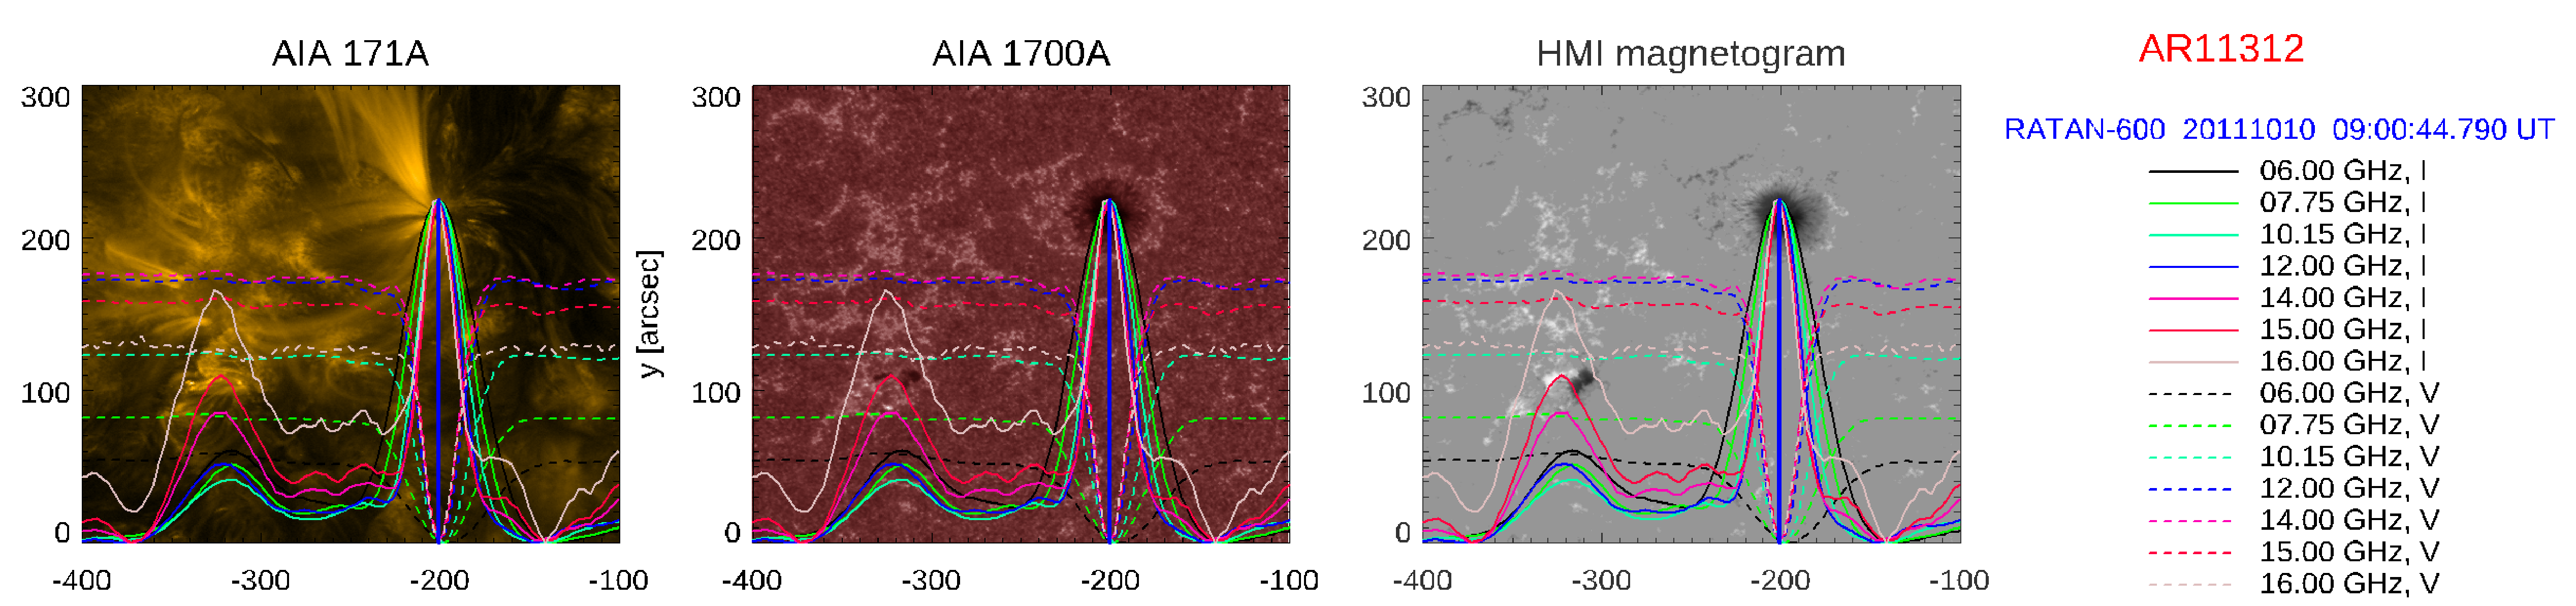
\includegraphics[width=0.99\textwidth]{images/20111010_AR11312_130044_ratan_sdo_0_az0.eps}
\caption{
Активная область AR11312 (10 октября 2011 г.). Слева направо: изображения SDO/AIA 171\,\AA, AIA 1700\,\AA\ и магнитограмма SDO/HMI. Цветными кривыми показаны одномерные сканы РАТАН-600 на выбранных частотах, указанных в легенде, совмещённые по пространственной координате с изображениями: сплошные линии --- Stokes~I, штриховые --- Stokes~V. Профили масштабированы по амплитуде к высоте панели; поляризационные профили (Stokes~V) дополнительно смещены по вертикали для наглядного разделения кривых.
}
	\label{ar11312_sdo_scans}
\end{figure*}

\subsection{Наблюдательные данные}
%{\todo
%\begin{itemize}
%  \item Радионаблюдения РАТАН-600: даты, частоты, разрешение.
%  \item Данные магнитного поля: SDO/HMI, восстановление NLFFF.
%\end{itemize}
%}

Для применения разработанного метода к реальным солнечным наблюдениям
была выбрана активная область NOAA~11312
(рис.~\ref{ar11312_sdo_scans}).
Область представляет собой сравнительно изолированное одиночное пятно
с простой, близкой к осевой симметрии структурой, что ранее определило
её выбор в качестве объекта анализа в работах
\cite{Stupishin2018,Alissandrakis2019}.
Благодаря морфологической простоте и отсутствию выраженной сложной
биполярной структуры NOAA~11312 является удобным тестовым объектом
для применения однородной модели, в которой атмосферные параметры
предполагаются зависящими только от высоты и усреднёнными по
поперечному сечению пятна. Это позволяет корректно сопоставлять
результаты различных диагностических подходов и использовать область
в качестве реперного случая для верификации алгоритма.

На изображениях SDO/AIA 1700\,\AA\ отчётливо выделяется  пятно (площадь $\sim 210$~ м.д.п.)

с симметричной полутенью, а в канале AIA 171\,\AA\ над пятном наблюдается
система корональных петель, локализованных преимущественно над его
центральной частью. Магнитограмма SDO/HMI демонстрирует доминирование
одной полярности в пределах пятна и слабые магнитные поля вне его,
что согласуется с характером круговой поляризации в микроволновых сканах.

Радионаблюдения выполнены 10 октября 2011 года на радиотелескопе
РАТАН-600 в диапазоне частот $3$\,--\,$18$~ГГц с  регистрацией параметров Стокса $I$ и $V$.
Пространственное разрешение РАТАН-600 в солнечных наблюдениях
является одномерным и определяется размерами диаграммы направленности,
которые зависят от длины волны. Размеры диаграммы направленности РАТАН-600 задаются соотношениями
$Q_{\mathrm{hor}}(\mathrm{arcsec}) = 0.85\,\lambda(\mathrm{mm})$
и
$Q_{\mathrm{vert}}(\mathrm{arcmin}) = 0.75\,\lambda(\mathrm{mm})$,
где $Q_{\mathrm{hor}}$ --- горизонтальный (вдоль сканирования),
а $Q_{\mathrm{vert}}$ --- вертикальный размер диаграммы,  $\lambda$ --- длина волны наблюдения в мм.  В рассматриваемом диапазоне частот это соответствует
горизонтальному разрешению от $\sim 15''$ (18~ГГц)
до $\sim 90''$ (3~ГГц). Одномерные сканы, совмещённые с ультрафиолетовыми изображениями
и магнитограммой, также приведены на рис.~\ref{ar11312_sdo_scans}.
Первичная обработка включала стандартную калибровку
и удаление фонового излучения спокойного Солнца.

Для моделирования микроволнового излучения использовался
фрагмент 
активной области из магнитограммы полного диска HMI.
Фотосферное магнитное поле экстраполировалось в приближении
нелинейного бессилового поля (NLFFF; \citealt{2023ApJS..267....6N}),
что позволило получить трёхмерную конфигурацию магнитного поля
над пятном, использованную при расчёте гирорезонансного излучения.


\subsection{  Формирование входного спектра и параметры моделирования}


 Положение максимума радиопотока определялось по скану на 15~ГГц. Значения потока в этой точке для всех частот и обеих круговых поляризаций формировали наблюдаемый микроволновый спектр, использованный в качестве входного вектора итерационного алгоритма.



На основе реконструированного магнитного поля и заданного начального приближения температурно--высотного профиля рассчитывались модельные одномерные сканы и применялась описанная выше в разделе %\ref{sec:iterations}
2.3
итерационная процедура.


Одним из ключевых параметров модели являлось произведение электронной концентрации на температуру в основании короны, $NT$, определяющее электронное давление и влияющее на распределение плотности по высоте. Значение $NT$ варьировалось в физически обоснованных пределах с целью достижения наилучшего согласия между модельным и наблюдаемым спектрами. Для каждого выбранного значения $NT$ итерационный алгоритм запускался независимо, после чего выбиралось решение, соответствующее минимальной остаточной невязке. 

\subsection{Результаты восстановления для активной области NOAA 11312}

Применение итерационного метода к наблюдениям активной области
NOAA~11312 позволило восстановить температурно-высотный профиль
атмосферы над солнечным пятном в рамках однородной модели.

На рис.~\ref{fig:AR11312R1P1} представлены восстановленные
температурные профили, а также модельные и наблюдаемые
микроволновые спектры в правой и левой круговых поляризациях.
Достигнуто хорошее согласие во всём диапазоне частот
3\,--\,18~ГГц; остаточная спектральная невязка не превышает
2.5\% как для каждой круговой поляризации по отдельности, так и для суммарного спектра.

\as{На рис.~\ref{fig:NTvar} показано .....
	В рассматриваемом случае оптимальное согласие достигалось при
	%\[
	%NT = 1 \times 10^{16}\ \mathrm{K\,cm^{-3}}.
	%\]
}

\begin{figure}
	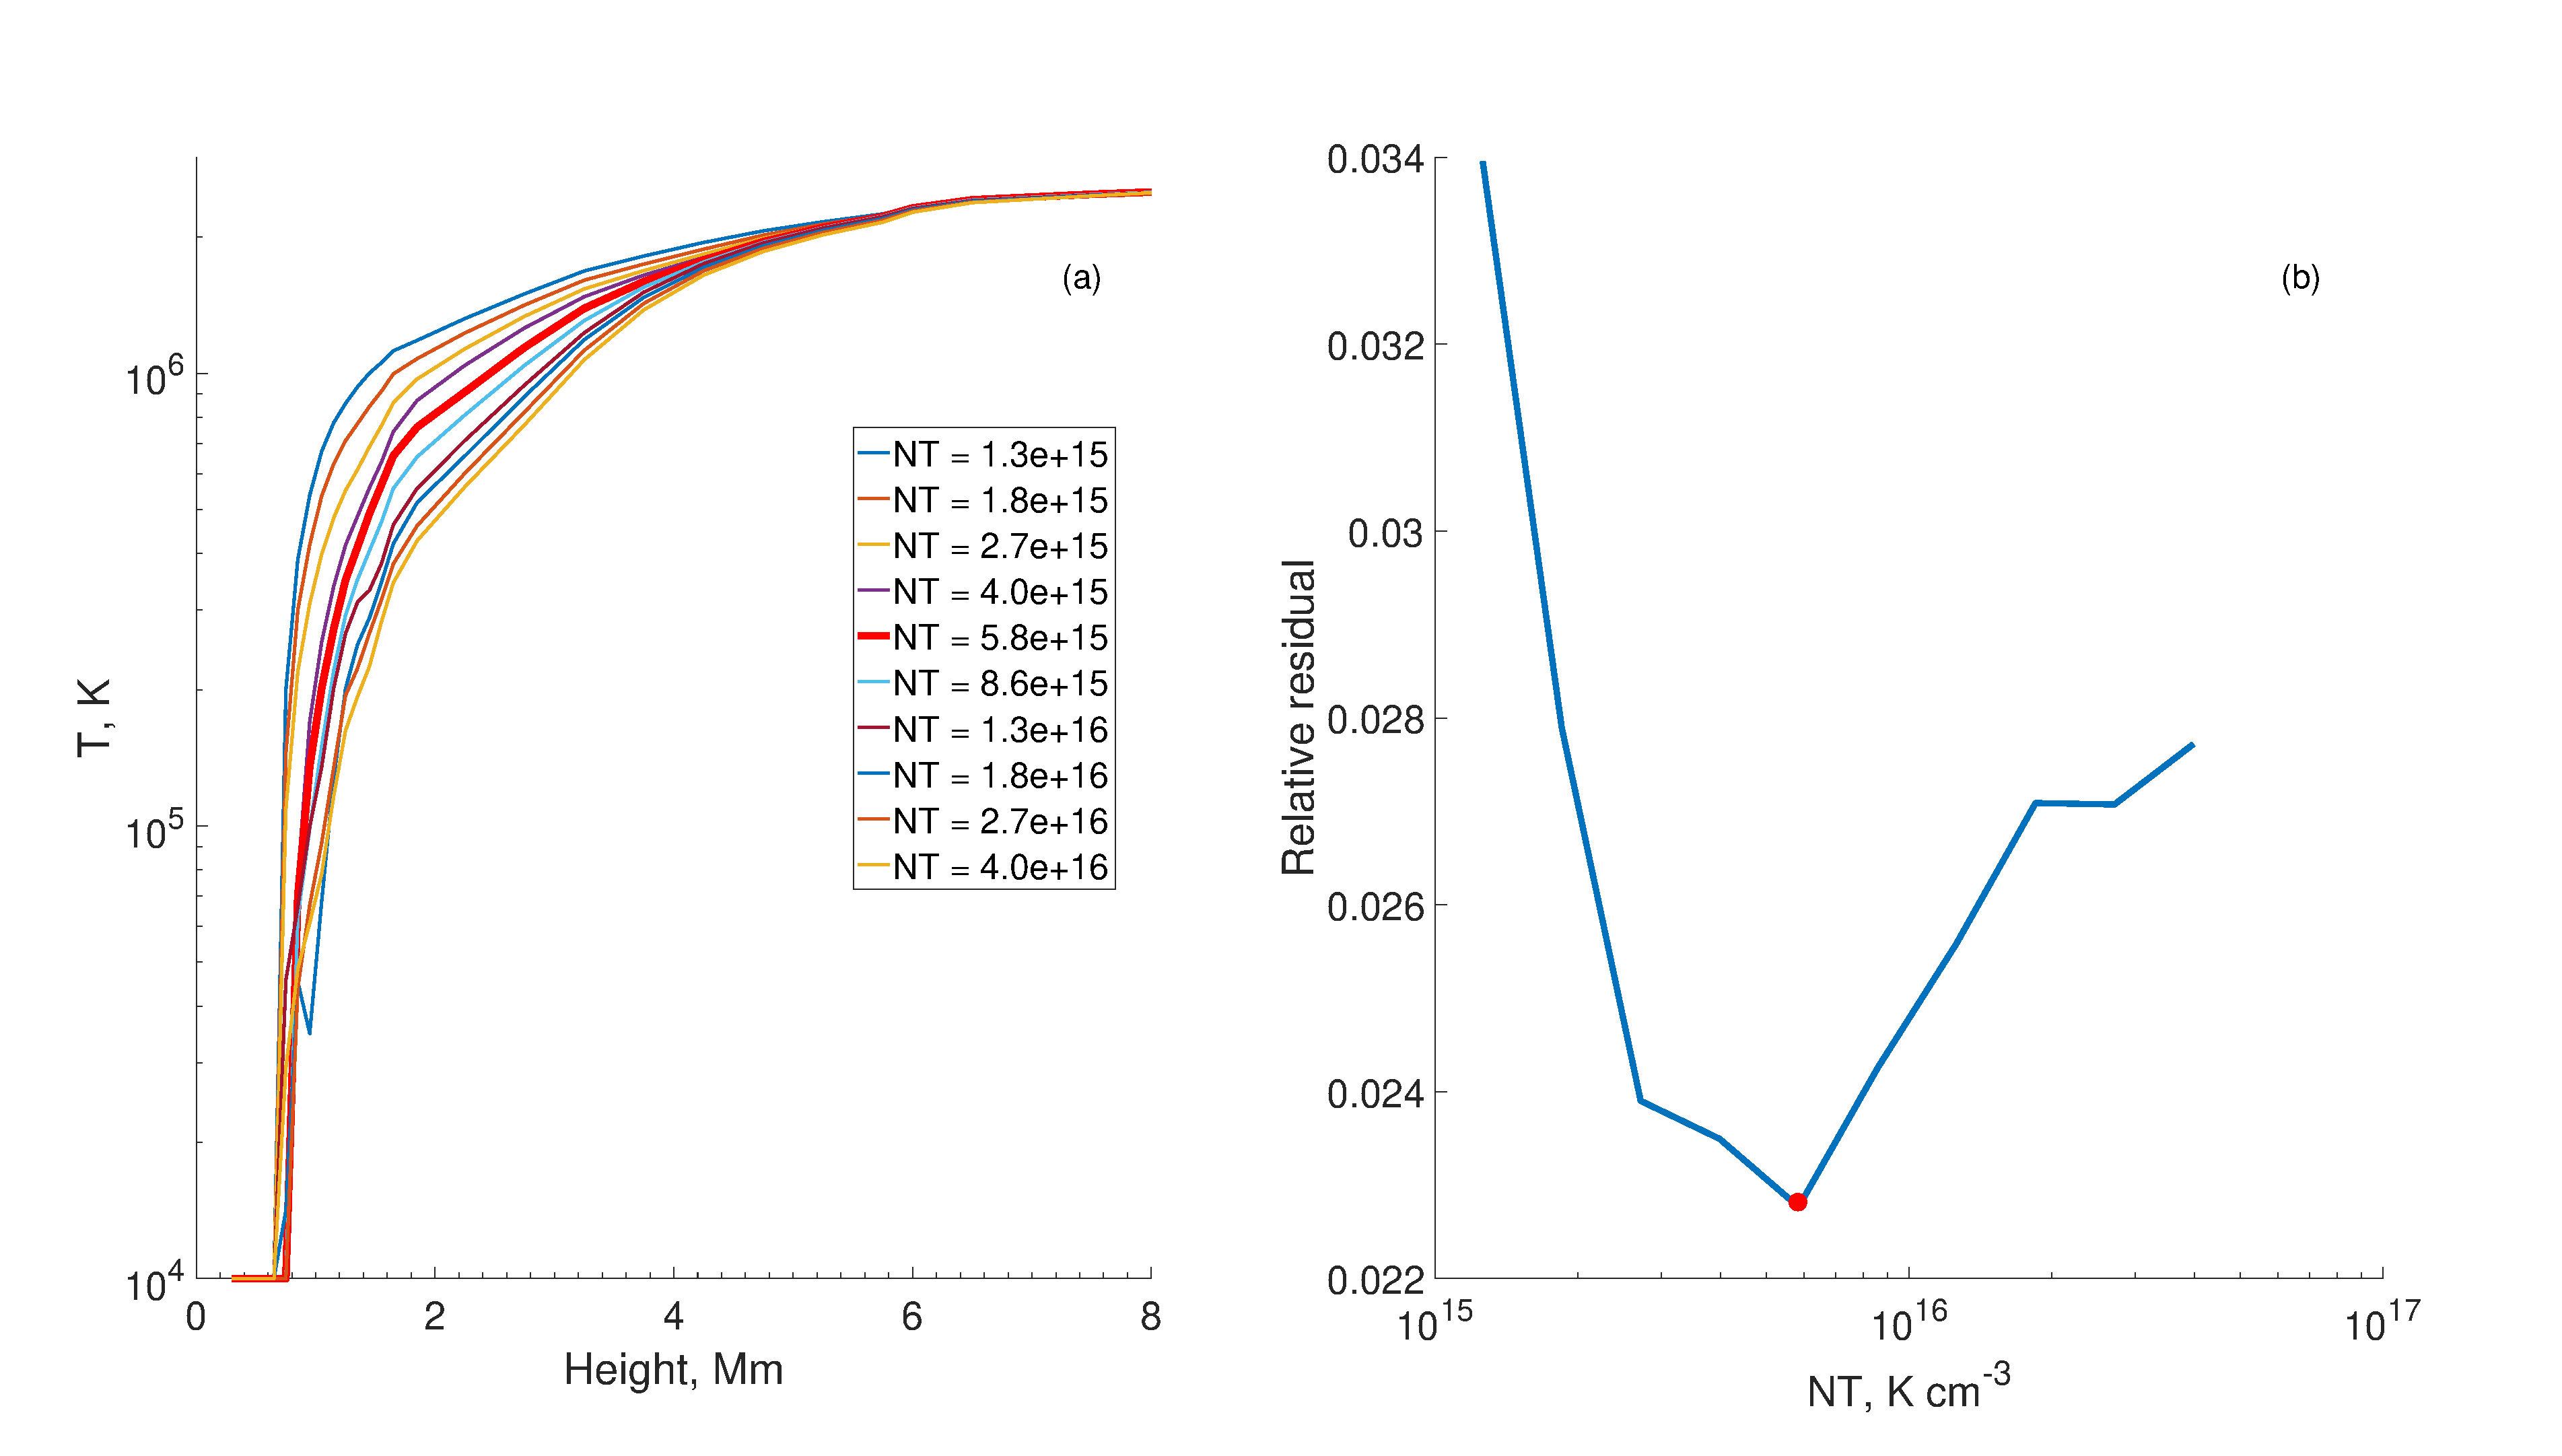
\includegraphics[width=1\linewidth]{images/NTvar2.eps}
	\caption{\as{Подбор NT.}}
	\label{fig:NTvar}
\end{figure}

Полученный профиль характеризуется значениями,
типичными для активных областей: 
 резкий рост температуры до корональных значений
наблюдается на высотах порядка 1.5\,--\,2~Mm.
Максимум  $2\times10^{6}$~K  достигается 
на высотах порядка 6\,--\,8~Mm.
Оценка электронной концентрации в низкой короне даёт
значения порядка нескольких $10^9$~$\mathrm{cm^{-3}}$, что соответствует ожидаемым параметрам атмосферы
над солнечными пятнами.

Проверка зависимости решения от выбора начального
приближения показала, что алгоритм сходится к близким
температурно-высотным профилям, что свидетельствует
о стабильности полученного решения.

\begin{figure}
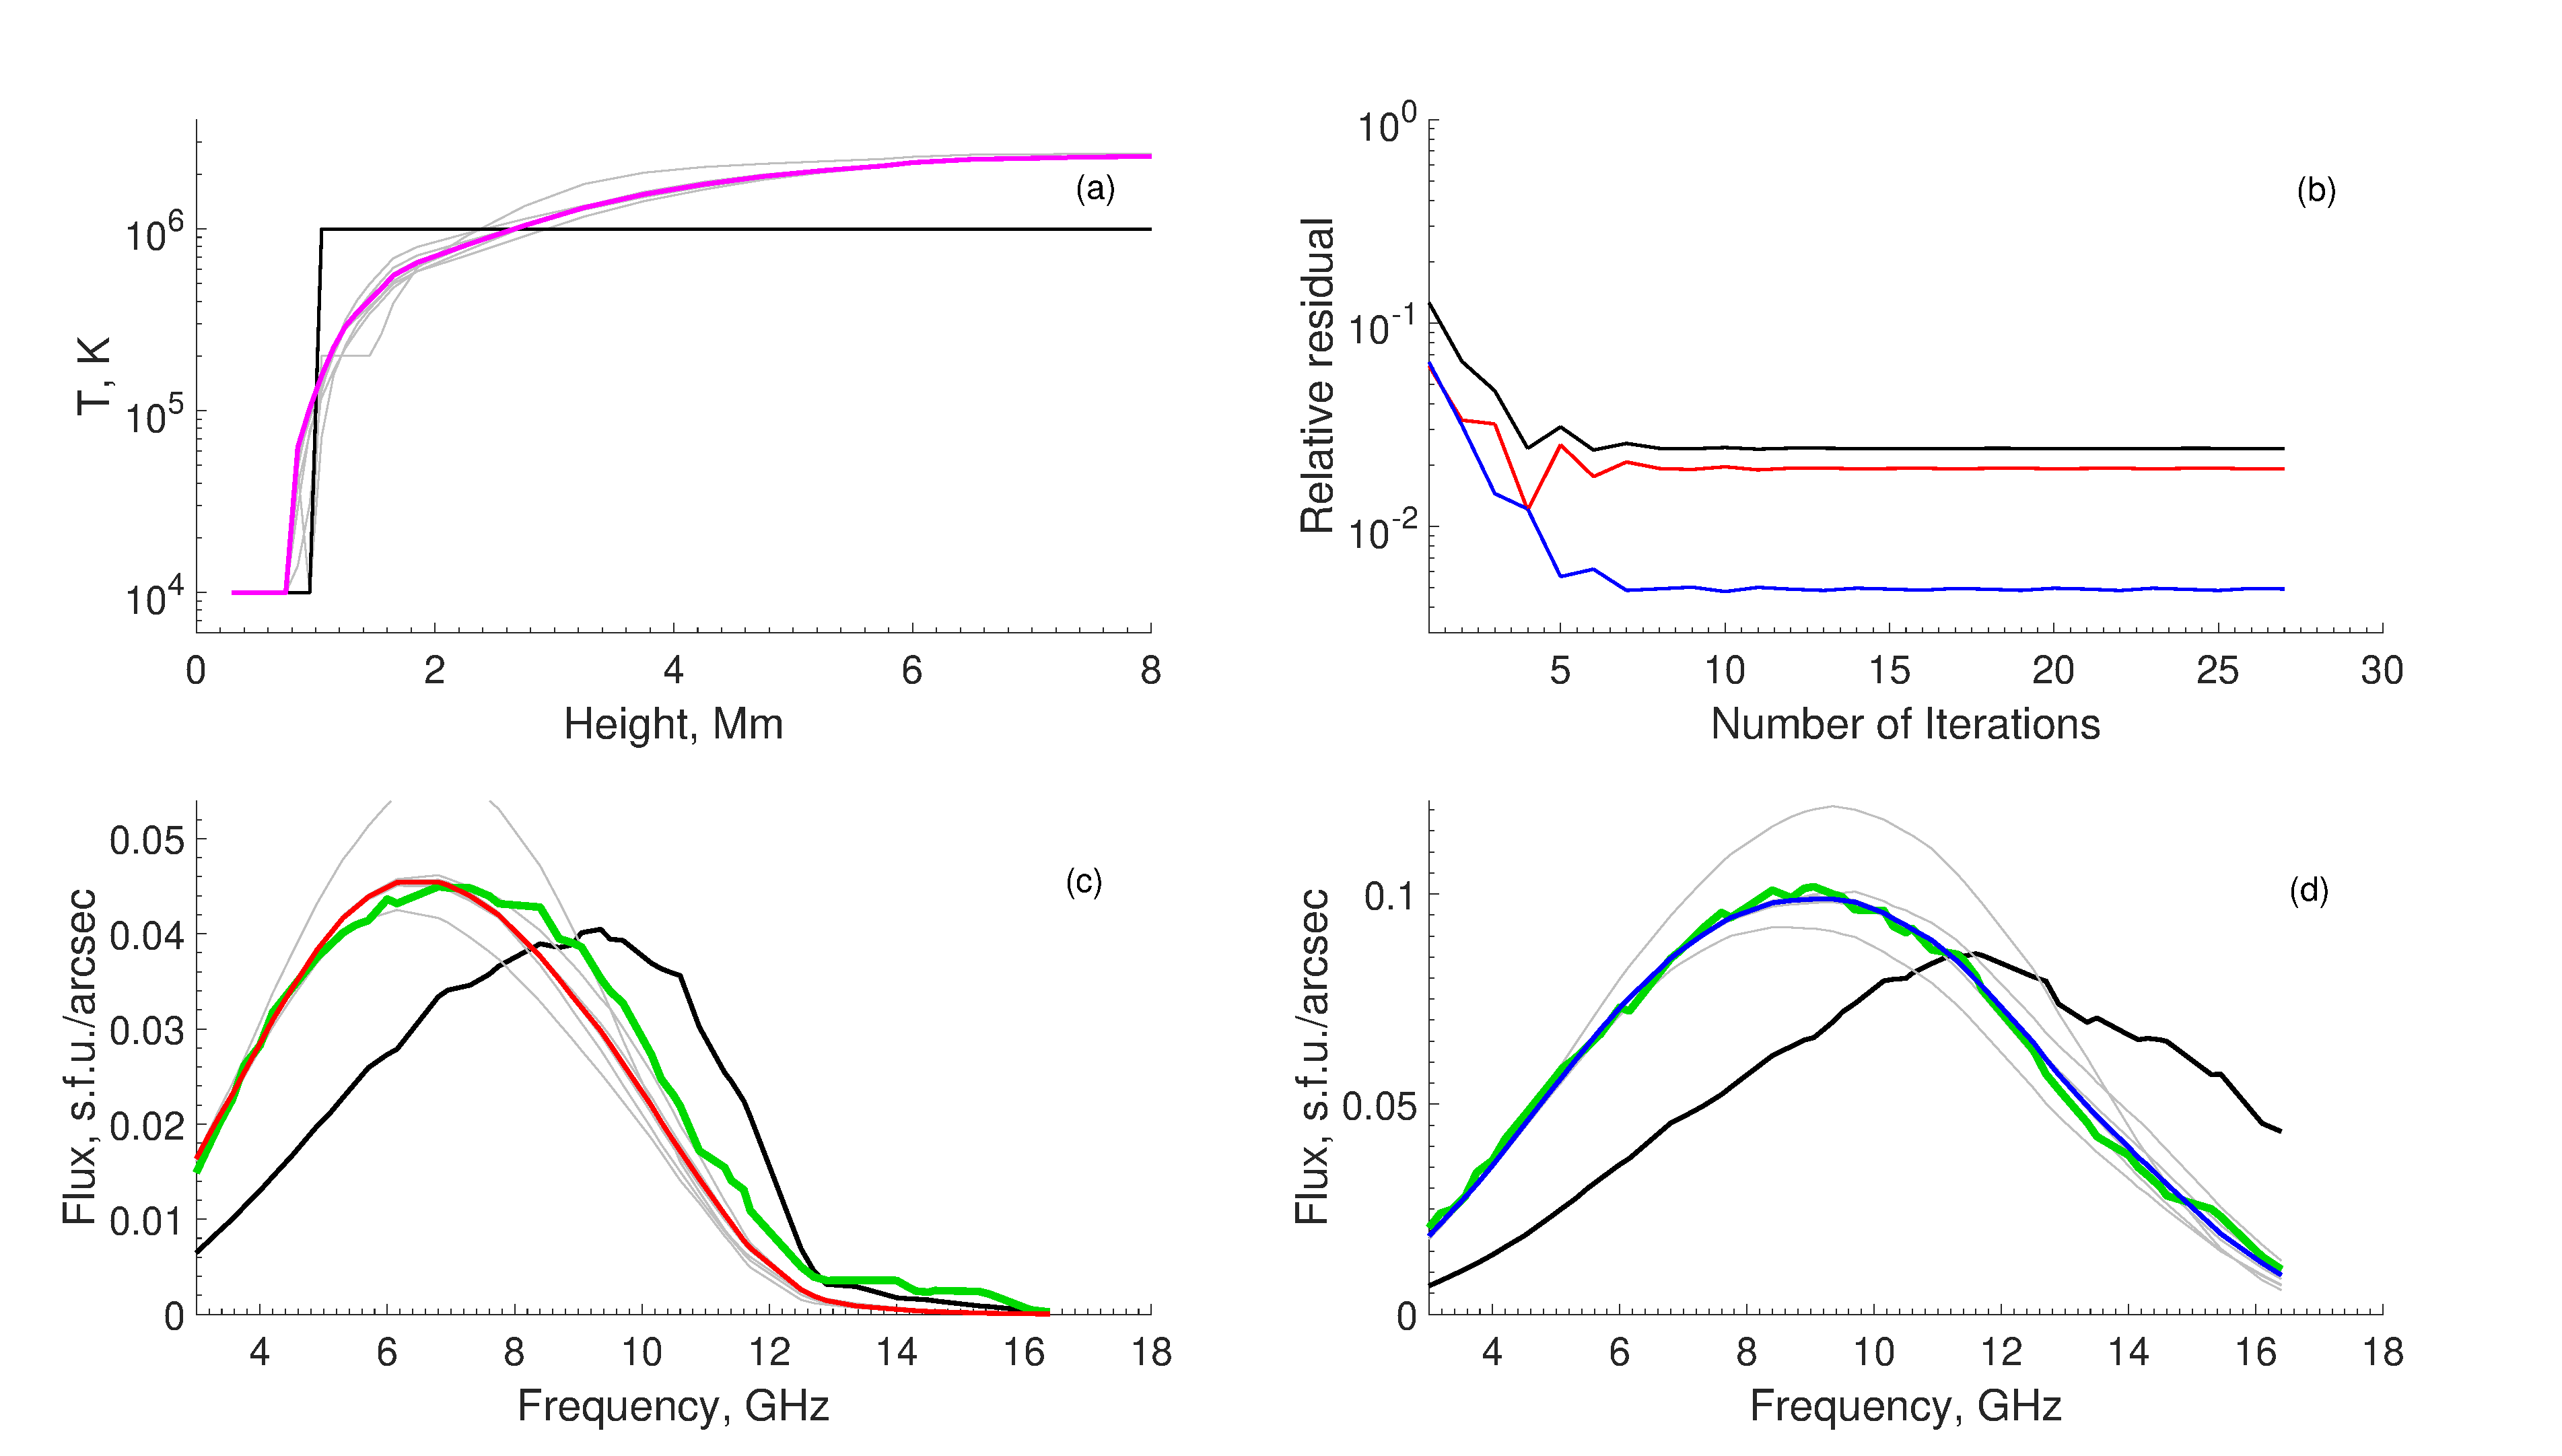
\includegraphics[width=1\linewidth]{images/AR11312R1P1_new.eps}
\caption{ Активная область NOAA 11312. Результат восстановления температурно-высотного профиля по спектру, сформированному в точке максимума одномерного скана. \as{Обозначения те же, что и на рис.~\ref{fig:Test}.}}
\label{fig:AR11312R1P1}
\end{figure}


\section{ОБСУЖДЕНИЕ}


%{\todo
%\subsection*{Достоверность и диагностические возможности однородной модели}
%\subsection*{Устойчивость и чувствительность метода}
%\subsection*{Ограничения }
%\subsection*{Сравнение с независимыми диагностическими подходами}
%    \subsubsection*{Сравнение с результатами \cite{Stupishin2018}}
%    \subsubsection*{Сравнение с DEM-моделированием \citep{Alissandrakis2019}}
%    \subsubsection*{Сравнение с полуэмпирическими моделями FAL}
%\subsection*{Перспективы развития метода}
%}


Тестирование алгоритма показывает, что однородная модель
обеспечивает устойчивое восстановление температурно-высотного
профиля с приемлемой точностью. В тестовых расчётах достигается
сходимость к заданному профилю, а для реальных данных ---
хорошее согласие модельных и наблюдаемых спектров.
Наибольшая диагностическая чувствительность реализуется
в диапазоне 6\,--\,15~ГГц, где гирорезонансное излучение
доминирует в формировании спектра. В этих условиях метод
позволяет восстанавливать структуру верхней переходной области
и нижней короны по микроволновым спектральным наблюдениям.

Анализ устойчивости показывает слабую зависимость решения
от начального приближения: даже при значительном смещении
исходного профиля сходимость сохраняется.
При добавлении шума до 3\,--\,5\% профиль восстанавливается корректно;
при более высоком уровне шума возрастает неопределённость
положения переходной области, однако корональные температуры
определяются надёжно. Параметр NT существенно влияет на форму
спектра, особенно в нижней короне, и может рассматриваться
как дополнительная диагностическая величина.

Вместе с тем следует учитывать ограничения метода.
Использование однородной модели приводит к усреднению структуры
тени и полутени. Вклад оптически тонкой компоненты ($F^{\mathrm{thin}}$),
особенно на высоких частотах, приводит к тому,
что излучение на фиксированной частоте формируется
не в окрестности одного слоя с $\tau_{\nu,p}\sim 1$,
а в протяжённом диапазоне высот ($\tau_{\nu,p}<1$).
В результате уменьшается высотная локализация
формирования сигнала и снижается чувствительность спектра
к температуре отдельных слоёв, что ухудшает обусловленность
задачи восстановления температурно-высотного профиля,
рассматриваемой в данной работе как обратная задача (инверсия спектра).
Дополнительную неопределённость вносит учёт теплового тормозного излучения, а также возможные погрешности реконструкции
магнитного поля.


Сопоставление с ранее опубликованными результатами,
полученными для той же активной области NOAA~11312,
демонстрирует согласованность оценок основных параметров.
Так,  в  работе \cite{Stupishin2018} были получены корональные температуры
1.5\,--\,2.5~MK и плотности порядка
$10^{9}$\,--\,$10^{10}\,\mathrm{cm^{-3}}$,
что согласуется с результатами настоящей работы.
Принципиальное отличие заключается в формализации задачи.
В настоящей работе инверсия сформулирована
в строгой матричной форме и сведена к решению
переопределённой системы линейных уравнений
с регуляризацией, что обеспечивает формальную
устойчивость решения, позволяет явно задавать
и варьировать вес регуляризующих условий,
количественно оценивать невязку и контролировать
сходимость, снижает зависимость результата
от выбора начального приближения и делает алгоритм
воспроизводимым и пригодным для систематического
применения к различным наблюдениям.
Предложенная схема также облегчает анализ
чувствительности решения к шумам и параметрам
дискретизации, что в предыдущей работе
не рассматривалось в явной форме.
Таким образом, реконструкция температурно-высотного
профиля переводится из эвристической итерационной
процедуры в строго формализованную задачу инверсии
с контролируемой устойчивостью решения,
что представляет собой существенное методическое
развитие подхода.

В работе \citep{Alissandrakis2019} та же активная область исследовалась
с использованием инверсии DEM по данным
SDO/AIA. В рамках DEM-подхода температурно-плотностная структура
восстанавливается при предположении стратификации и гидростатического
равновесия; высотная шкала формируется интегрированием уравнений
гидростатики при заданных граничных условиях. DEM-модели удовлетворительно
воспроизводят наблюдаемые микроволновые спектры, однако реконструкция
ограничена диапазоном температур, чувствительных к каналам AIA, и требует
модельного задания нижней границы переходной области.

В настоящей работе высотная привязка излучающих слоёв определяется
непосредственно условиями гирорезонансного формирования излучения
через распределение магнитного поля, что обеспечивает независимую
диагностику верхней переходной области и коронального плато температуры.
Таким образом, оба подхода основаны на различных физических предпосылках
и используют разные диагностические механизмы.


Сравнение полученного температурно-высотного профиля
с полуэмпирическими моделями серии FAL \citep{Fontenla2009}
показывает, что основные параметры находятся в согласии
с типичными характеристиками активных областей:
положение переходной области и уровень корональных температур
соответствуют диапазонам, приводимым в этих моделях.


Следует учитывать, что модели FAL основаны на инверсии
ультрафиолетовых и рентгеновских спектральных линий,
формирующихся в условиях NLTE и нередко обладающих
значительной оптической толщиной. В этом случае
наблюдаемое излучение не является прямой функцией
локальной температуры плазмы, а определяется полной
задачей переноса излучения, включающей поглощение,
переизлучение и перераспределение фотонов по частоте
и высоте. Температурно-высотные профили FAL представляют
собой результат решения NLTE-задачи, в которой
распределения температуры и плотности подбираются
для воспроизведения наблюдаемых спектральных линий.

В микроволновом диапазоне излучение носит 
непрерывный характер и формируется в условиях,
близких к локальному термодинамическому равновесию.
Яркостная температура в слое с оптической толщиной
порядка единицы непосредственно связана с электронной
температурой плазмы, что позволяет более прямо
интерпретировать наблюдения. Таким образом,
микроволновая диагностика и NLTE-моделирование
спектральных линий представляют собой два принципиально
различных и комплементарных подхода к восстановлению
термодинамической структуры солнечной атмосферы.


Перспективы развития метода  связаны с расширением модели
за пределы одномерного усреднения. Прежде всего, реальная структура солнечного пятна является
неоднородной и включает  различные зоны (пятно с тенью и полутенью,  окружающие флоккулы и т.д.),
обладающие различными магнитными и термодинамическими
характеристиками.

Используемая в работе усреднённая параметризация
может быть расширена до раздельного описания этих областей.
Дополнительное использование нескольких точек скана
позволит пространственно разделить вклады различных
частей пятна и перейти от одномерного усреднения
к более реалистичному описанию его структуры. Естественным дальнейшим шагом является применение метода
к двумерным картам яркостной температуры,
полученным на интерферометрических радиотелескопах,
что позволит отказаться от осевой симметрии
и реализовать пространственно разрешённую
инверсию температурно-высотной структуры.

Другим направлением развития является более строгий учёт
радиационного переноса, включая корректное описание
вклада тормозного (free--free) излучения.
На длинных волнах его роль возрастает вследствие увеличения
коэффициента поглощения с длиной волны.
В области коротких волн условие гирорезонансного формирования
излучения для низких гармоник требует более высоких значений
магнитного поля; если такие значения не достигаются
на соответствующих высотах, относительный вклад
free--free-компоненты увеличивается.
Таким образом, на обоих краях микроволнового диапазона,
а также в частотных интервалах с ослабленным гирорезонансом,
корректный учёт тормозного излучения является необходимым
для точного восстановления температурно-высотного профиля,
особенно в корональной части.

Наконец, сопоставление результатов микроволновой инверсии
с независимыми диагностическими методами, в частности
с DEM-анализом по данным EUV-наблюдений, представляется
перспективным направлением дальнейших исследований.
Поскольку данные подходы основаны на различных механизмах
формирования излучения, их согласованное применение
способствует формированию более целостного представления
о температурно-высотной структуре активных областей.


\section{ЗАКЛЮЧЕНИЕ}

В работе выполнено развитие и формализация итерационного метода
восстановления температурно-высотного профиля солнечной атмосферы
по многочастотным микроволновым наблюдениям. В отличие от ранее
использовавшейся схемы, задача решена в виде формализованной
инверсии переопределённой системы линейных уравнений
с регуляризацией, что обеспечивает устойчивость,
контролируемость и воспроизводимость решения.

Численные тесты на синтетических данных продемонстрировали
устойчивую сходимость алгоритма и его поведение при наличии шумов.
Применение метода к наблюдениям активной области NOAA~11312
(РАТАН-600, диапазон 3\,--\,18~ГГц) позволило восстановить
температурно-высотный профиль с корональными температурами
порядка $(2.0$\,--\,$2.4)\times10^{6}$~К при хорошем согласовании
модельных и наблюдаемых спектров.

Сопоставление с опубликованными результатами,
полученными независимыми диагностическими подходами,
показывает согласие по основным характеристикам
температурной структуры в области переходной зоны
и нижней короны. Используемое однородное приближение
определяет пределы интерпретации полученного профиля
и задаёт направления дальнейшего совершенствования метода.


\begin{acknowledgments}
{Наблюдения на телескопах САО РАН выполняются при поддержке Министерства науки и высшего образования Российской Федерации. Обновление приборной базы осуществляется в рамках национального проекта «Наука и университеты».  

Авторы также благодарят команду проекта SDO за возможность использования данных, полученных с помощью этого инструмента.
}
\end{acknowledgments}

\section*{ФИНАНСИРОВАНИЕ}
{ Работа  выполнена в рамках государственного задания САО РАН, утвержденного Министерством науки и высшего образования Российской Федерации. 
}

\section*{КОНФЛИКТ ИНТЕРЕСОВ}
Авторы заявляют об отсутствии конфликта интересов.


\newcommand{\ssr}{Space Science Reviews }

\bibliographystyle{aspb1}
\bibliography{Paper}
\end{document}